\documentclass[twocolumn, times]{aastex61}


\usepackage{underscore}
% alternate micron command
\newcommand{\um}{\micron}

% referencing commands
\newcommand{\sref}[1]{Sec.~\ref{#1}}

\usepackage[T1]{fontenc}

% commands and packages that shouldn't be needed in final version
\usepackage{xcolor, soul}


\newcommand{\ascl}[1]{\href{http://www.ascl.net/#1}{ascl:#1}}
\newcommand{\status}[1]{\textsf{#1}}
\newcommand{\jyas}{Jy\,arcsec\textsuperscript{$-$2}}
\newcommand{\jybm}{Jy\,beam\textsuperscript{$-$1}}

\hypersetup{bookmarks=true}

\shorttitle{JCMT LR: SCUBA-2 850\micron}
\shortauthors{SF Graves et al.}


\begin{document}
\title{The JCMT Legacy Release: SCUBA-2 850\micron\ Coadds and Catalogs}

\author{Sarah F. Graves}
\affiliation{East Asian Observatory, 660 N.\ A`oh\=ok\=u Place, Hilo, HI 96720, USA}
\affiliation{Joint Astronomy Centre, 660 N.\ A`oh\=ok\=u Place, Hilo, HI 96720, USA}
\author{Graham S. Bell}
\affiliation{East Asian Observatory, 660 N.\ A`oh\=ok\=u Place, Hilo, HI 96720, USA}
\affiliation{Joint Astronomy Centre, 660 N.\ A`oh\=ok\=u Place, Hilo, HI 96720, USA}
\author{David S. Berry}
\affiliation{East Asian Observatory, 660 N.\ A`oh\=ok\=u Place, Hilo, HI 96720, USA}
\affiliation{Joint Astronomy Centre, 660 N.\ A`oh\=ok\=u Place, Hilo, HI 96720, USA}
\author{Iain M. Coulson}
\affiliation{East Asian Observatory, 660 N.\ A`oh\=ok\=u Place, Hilo, HI 96720, USA}
\affiliation{Joint Astronomy Centre, 660 N.\ A`oh\=ok\=u Place, Hilo, HI 96720, USA}
\author{Malcolm J. Currie}
\affiliation{RAL Space, Rutherford Appleton Laboratory, Harwell Campus, Didcot OX11 0QX, UK}
\affiliation{Joint Astronomy Centre, 660 N.\ A`oh\=ok\=u Place, Hilo, HI 96720, USA}
\author{Jessica T. Dempsey}
\affiliation{East Asian Observatory, 660 N.\ A`oh\=ok\=u Place, Hilo, HI 96720, USA}
\affiliation{Joint Astronomy Centre, 660 N.\ A`oh\=ok\=u Place, Hilo, HI 96720, USA}
\author{Per Friberg}
\affiliation{East Asian Observatory, 660 N.\ A`oh\=ok\=u Place, Hilo, HI 96720, USA}
\affiliation{Joint Astronomy Centre, 660 N.\ A`oh\=ok\=u Place, Hilo, HI 96720, USA}
\author{Tim Jenness}
\affiliation{To be assigned}
\affiliation{Joint Astronomy Centre, 660 N.\ A`oh\=ok\=u Place, Hilo, HI 96720, USA}
\author{Doug Johnstone}
\affiliation{NRC Herzberg Institute of Astrophysics, 5071 West Saanich Rd, Victoria, BC, V9E 2E7, Canada}
\affiliation{Department of Physics and Astronomy, University of Victoria, Victoria, BC, V8P 1A1, Canada}
\affiliation{Joint Astronomy Centre, 660 N.\ A`oh\=ok\=u Place, Hilo, HI 96720, USA}
\author{Harriet A. L. Parsons}
\affiliation{East Asian Observatory, 660 N.\ A`oh\=ok\=u Place, Hilo, HI 96720, USA}
\affiliation{Joint Astronomy Centre, 660 N.\ A`oh\=ok\=u Place, Hilo, HI 96720, USA}
\author{Mark G. Rawlings}
\affiliation{East Asian Observatory, 660 N.\ A`oh\=ok\=u Place, Hilo, HI 96720, USA}
\author{Holly S. Thomas}
\affiliation{Joint Astronomy Centre, 660 N.\ A`oh\=ok\=u Place, Hilo, HI 96720, USA}
\affiliation{SMA/Harvard}
\author{Jan G. A. Wouterloot}
\affiliation{East Asian Observatory, 660 N.\ A`oh\=ok\=u Place, Hilo, HI 96720, USA}
\affiliation{Joint Astronomy Centre, 660 N.\ A`oh\=ok\=u Place, Hilo, HI 96720, USA}

\correspondingauthor{Sarah F. Graves}
\email{s.graves@eaobservatory.org}

\begin{abstract}
  We present the JCMT Legacy Release, consisting of uniform
  reductions, coadds, and catalogs of detected emission for the
  850\,\um\ data from all SCUBA-2 observations taken between 2011
  February 2 and 2015 March 1. The data are gridded onto HEALPix tiles
  of $\approx$1 degree a side, using the HPX projection with pixels of size
  $\approx$3.22 arcseoncds. The individually reduced observations
  include 6420 hours of observing time, and the coadds tiles used 5828
  hours of this, covering 1356 square degrees of the sky. The coadds
  have been calibrated into units of m\jyas\ using a single,
  self-derived flux conversion factor of 2.46 Contiguous regions of
  emission were detected at a better than 5-$\sigma$ level in 740
  tiles, covering in total 1.4 square degrees, or 0.10 percent of the
  coadded area. Within this area, 13477 local maxima were
  detected. Sixteen of the coadded tiles contain regions with a noise
  better than 1\,m\jybm. The coadds and catalogues can be found at
  CADC at:
  \url{http://www.cadc-ccda.hia-iha.nrc-cnrc.gc.ca/en/search/?Observation.proposal.id=JCMT-LR}

WHat its point is \& how you get it.
\end{abstract}

\keywords{catalogs; submillimeter:general}

\section{Introduction}
\label{sec:intro}
% JCMT & SCUBA-2 & JSA
The James Clerk Maxwell Telescope (JCMT) is a 15-m submillimetre
telescope located at an altitude of 4092\,m on Maunakea, where it has
been operating since 1987. Its current instrument suite includes
SCUBA-2 (Submillimetre Common User Bolometer Array 2), a 10,000-pixel
continuum camera that observes simultaneously at 450\,\um\ and
850\,\um\ wavelengths \citep{Holland2013}, and has been operating in
full science mode since February 2011.

% why this release
To maximise the scientific return of these many years of archival
data, and to make it as easy as possible for non-submm-experts to use
the JCMT data, the Joint Astronomy Centre (JAC), then-operators of the
JCMT, decided to produce `legacy' reductions of all public data from
the current instrumentation. This work has been continued since 2015
March by East Asian Observatory (EAO), the current operators of the
JCMT. These legacy reductions are envisioned as providing a uniform,
standardized reduction, coadds, and emission detection of all publicly
available observations, regularly updated as more observations become
public. The aim has been to produce uniformly reduced high-quality
coadds maps that required as little checking as possible by eye, and
which would allow astronomers to easily discover which regions have
been observed, the noise levels in existing regions, and where there
are clear detections. Previously, the SCUBA Legacy Catalog
\citep{DiFrancesco2008} presented uniformly reduced coadds and
catalogs of much of the public SCUBA data, and this resource has been
very widely used.

The first product of the legacy release project, the JCMT legacy
release (LR1) was made public in September 2015, and included
850\micron\ SCUBA-2 data from 2011 February 2 to 2013 August 1. This
paper presents the expanded and updated LR2 release, including SCUBA-2
850\micron\ data from 2011 February 2 to 2015 March 1st. This covers
all observations taken before the handover of the JCMT from JAC to
EAO. For simplicity, we will refer to the current release as the LR.
It is expected that the 850um legacy release will be regularly updated
with new versions in thefuture as more SCUBA-2 data is taken and
becomes public.

Planned future releases are the 450\,\um\ SCUBA-2 observations and
HARP spectral cubes, as well as regular updates to the 850\,\um\
release.

% Added back in -- oculd be shorter, but description and citation of
% JSA needs to go somwhere.
This data release is publicly accessible and fully queryable by sky
position through the JCMT Science Archive \citep[JSA]{2015Economou},
hosted at the Canadian Astronomy Data Centre (CADC). This archive also
hosts our proprietary (with authentication) and public raw
observations and our standard pipeline reduced products. Unlike the
LR, the normal reductions do not include full coadds of data taken on
different nights. In addition, these observations from different projects
may have been reduced with different configurations and can not be
naively coadded.



% % Release of block 1 and these data
% This release includes data taken from 2011 February 2 to 2015 March
% 1st, when the JCMT was began to be operated by East Asian Observatory.
% The first block of these data, from 2011 to 2013 August 1 was already
% reduced and publicly released in September 2015. This release includes
% these same reduced individual observations, reductions of the newer
% data taken up until March 2015, and new co-adds and catalogs produced
% from all the data (and using a slightly different calibration
% constant).
\begin{figure}
  \centering
  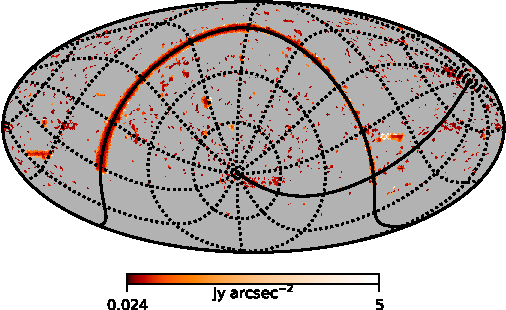
\includegraphics{mollweide-average-noise-galacticaxes-crop}
  \caption{All-sky noise map for this SCUBA-2 850\,\um{} legacy
    release. Each pixel represents the average noise across a single
    HEALPix tile. Tiles with fewer than 200 valid pixels were not
    included. The map is a Cartesian Mollweide projection, with the
    axes of the galactic coordinate system overlaid. The large curved
    stripe shows the extensive mapping of the Galactic Plane. Small
    points away from the plane predominantly represent small scanning
    (DAISY) observations towards extragalactic sources scattered
    across the sky.}
  \label{fig:noise-mollweide}
\end{figure}

\subsection{Outline of paper}

This paper presents first in section \ref{sec:overview} a summary of
the release and the included observations, various overall statistics
and some details on the noise properties of the release. Section
\ref{sec:examples} shows the scientific products created towards three
example regions (chosen to cover a range of different astronomical
objects). Section \ref{sec:healpix} describes the HEALPix grid used in
this release, and then Section \ref{sec:dr} describes our data
reduction procedures. We describe the calibration of these maps
in Section \ref{sec:calib}, including a discussion of some of the more
subtle effects of the data reduction method used. Section
\ref{sec:cat} then describes the emission catalogs. We finish by
summarizing the pointing offsets found in Section \ref{sec:pointing},
and the beam shape in Section \ref{sec:beam}.

\section{Overview of Release}
\label{sec:overview}
This release includes publicly released 850\,\um\ science observations
observed between 2011 February 2 and 2015 March 1, including
observations from calibration projects, PI projects, and the JCMT
Legacy Surveys (JLS). See \citealt{ChrysostomouJLS} for an overview of
the JCMT Legacy Survey program, which included SCUBA-2 observations
for: the Gould Belt Survey \citep{GBS}, the SCUBA-2 ambitious Sky
Survey \citep{SASSy}, the Cosmology Legacy Survey \citep{Geach2013},
the JCMT Galactic Plane Survey \citep{JPS}, the Nearby Galaxy Survey
\citep{NGLS}, and the Debris Disk Survey \citep{SONS}.  Observations from
earlier than 2011 February 2 were not included, as these were taken in
\emph{shared risk} mode while instrument commissioning was still being
conducted, and the data from that era are more problematic
\citep{SC19,Dempsey2010}. The first block of the released data, from
2011 to 2013 August 1 (but not including the Cosmology Legacy Survey
(CLS) observations) was previously reduced and publicly released in
September 2015, using the same configuration and coadd criteria as
described in this paper, but calibrated using a slightly different
flux conversion factor (FCF).


For these observations, we have produced individual reduced
observations, coadds of all science observations that fell on a given
tile, and catalogs of extended contiguous regions and local peaks
detected at $>5\sigma$. Fig.\,\ref{fig:noise-mollweide} shows the
all-sky noise map of the coadds in this release, showing the average
RMS across all valid pixels in a tile as a single square.

All pointing and science observations from our time range, excluding
Solar System objects/moving targets, were reduced using the ORAC-DR
\citet{2015oracdr} recipe
\texttt{REDUCE\_SCAN\_JSA\_PUBLIC}\footnote{ORAC-DR is the data
  reduction pipeline used at the JCMT} onto our tiles, using the HPX
projection (see Section \ref{sec:healpix}). These reduced maps are in
the instrumental units of pW (see Section \ref{sec:dr}). The
individual-observation maps are available to download through the JSA,
where they are listed under their original project code and
metadata. Pointing observations were not used or analysed further in
this release. We also excluded solar system objects/moving targets
from this release.


All the reduced science observations were individually examined to
determine if they met our quality standards (see Section
\ref{sec:QA}). Coadds were then made for every tile with data
falling onto it, using the recipe \texttt{COADD\_JSA\_TILES}
(see Section \ref{sec:coadd}), producing a coadded tile calibrated in
units of m\jyas{} (for details of the calibration see
Section~\ref{sec:calib}). For every coadded tile, the recipe
\texttt{JSA\_CATALOGUE} was then run to produce (if detected) extent
and peak catalogs of detected emission (see Section
\ref{sec:cat}).

% \begin{figure}
%   \centering
%   \includegraphics[width=1.0\linewidth]{flowchart2}
%   \caption{Vizualisation of the flow of observations through the
%     processing system and into the final tile based products. Here, 8
%     of the input observations into tile\,3311 are shown at the
%     top. These were reduced using REDUCE\_JSA\_PUBLIC, and split up
%     onto our tiles. Red boxes indicate the part of the observation
%     that fell onto this tile (3311) -- note that a large PONG
%     observation will typically fall onto many of our tiles. A red 'X'
%     over the top right observation indicates that it was judged as
%     'BAD' during the Quality Assurance (QA) analysis (in this case,
%     due to strange noise features in the background and a `scuff' of
%     bright emission one one edge of the scan). It was not included in
%     further processing. The other observations were then combined with
%     COADD\_JSA\_TILES to produce the coadded tile shown in the bottom
%     left. JSA\_CATALOGUE was then used to create an extent catalogue
%     and a peak catalogue; the preview images for these files are shown
%     in the bottom right, with the catalogue regions outlined in
%     red. The images shown in this flowchart are taken from the preview
%     images produced by our processing system, and visible at CADC when
%     searching this release.}
%   \label{fig:flowchart}
% \end{figure}


% add note -- available at (URL for download)
%\note{Has any NGLS SCUBA-2 data been published (NO)? Need need proper
%  SASSy refs. (There are none better as far as we know...)}


The observations included in this release were each taken in one of
the two different SCUBA-2 standard scan patterns: CV\_DAISY (hereafter
DAISY), a fixed-size scan pattern used for covering small areas, and
CURVY\_PONG (hereafter PONG) scan patterns at various user-chosen
sizes, used for covering larger areas \citep{Holland2013}.  The
scanning speed is not the same between these scan patterns; this will
cause some inconsistency in the scales of emission detected in the
reduced maps, as SCUBA-2 observations are sensitive to different size
scales of emission at different speeds. However, our reduction has
been extremely conservative and has filtered out structure on scales
larger than 200\arcsec, so this difference will be minimized in our
coadds.



\subsection{Anticipated uses}

\subsection{Accessing the release}

\subsection{Overall statistics of the release}

In total, 21464 observations were reduced representing 6420 hours of
observing time, towards 4403 distinct tiles. The coadded observations
include 12404 science and calibration observations which passed QA
(5828 hours or 242.8 days) towards 4151 tiles. These coadds were made
up of 136 hours of science calibration observations, 3575 hours of
data taken for the JCMT Legacy Surveys and 2117 hours of data taken
for PI projects. This information is summarized in Table
\ref{tab:typesobs}. The coadds include 1.69 gigapixels of valid data,
corresponding to $\approx$ 1356 square degrees. For comparison, the
SCUBA Legacy Catalog \citep{DiFrancesco2008} covered 19.6 square
degrees in their `Fundamental Map Data Set, and 29.3 square degrees in
their fuller `Extended Map Data Set'.

\begin{deluxetable}{lrrr|rrr}

  \tablecaption{Types of observation included in this release.\label{tab:typesobs}}
  \tablecolumns{7}
  \tablehead{
    & \multicolumn{3}{c}{Indiv. Obs} & \multicolumn{3}{c}{Coadds}\\
    \cline{2-4} \cline{5-7}
    \colhead{Type} & \multicolumn{1}{p{0.75cm}}{Num. obs.} & \multicolumn{1}{p{0.75cm}}{Time (h)} & \colhead{Tiles} & \multicolumn{1}{p{0.75cm}}{Num. obs.} & \multicolumn{1}{p{0.75cm}}{Time (h)} & \colhead{Tiles}}
  \startdata
All & 21464 & 6420.0 & 4403 & 12404 & 5828.1 & 4151 \\
Sci. & 12594 & 5914.5 & 4185 & 12404 & 5828.1 & 4151 \\
Pointing & 8870 & 505.5 & 292 & 0 & 0.0 & 0 \\
Calib. & 2234 & 138.1 & 22 & 2200 & 135.9 & 22 \\
JLS & 6143 & 3642.2 & 2156 & 6023 & 3575.3 & 2145 \\
PI & 4217 & 2134.2 & 2329 & 4181 & 2117.0 & 2303\\
\enddata
\end{deluxetable}

Emission detection was carried out on all of the coadded tiles, and
this resulted in detections in 1.37 square degrees
($4.17\times10^{-4}$ steradians), or 0.10\% of the area observed).


\begin{deluxetable}{rDDD}
  \tablecaption{Areas of the release with an RMS noise less than or
    equal to the given value. \label{tab:noises}}
  \tablehead{\colhead{RMS} &
    \multicolumn{2}{p{1.6cm}}{Equivalent} &
    \multicolumn{2}{p{1.25cm}}{\centering Area} &
    \multicolumn{2}{p{1.25cm}}{\centering Fraction}\\
    \colhead{\centering $\mathrm{mJy\,beam^{-1}}$} &
    \multicolumn{2}{p{1.5cm}}{\centering $\mathrm{mJy\,arcsec^{-2}}$}&
    \multicolumn{2}{p{1.25cm}}{\centering $\mathrm{{}deg^{2}}$} &
    \multicolumn{2}{p{1.25cm}}{$ $}}

  \decimals
  \startdata
  1.0 & 0.0043 & 0.1819 & 0.00013 \\
  2.0 & 0.0086 & 0.8075 & 0.0006 \\
  10.0 & 0.043 & 44.76 & 0.033 \\
  25.0 & 0.107 & 176.7 & 0.13 \\
  50.0 & 0.215 & 331.6 & 0.24 \\
  100.0 & 0.431 & 1043 & 0.77 \\
  200.0 & 0.862 & 1277 & 0.94 \\
  \enddata
\end{deluxetable}

\begin{figure}
  \centering
  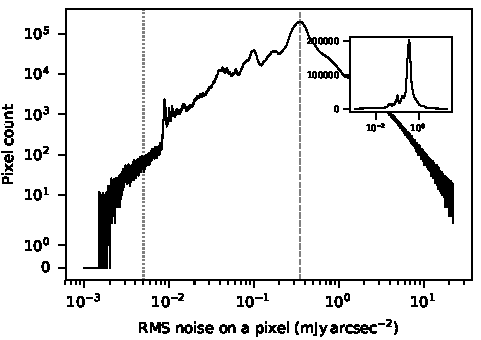
\includegraphics{coadds-noise-histogram.pdf}
  \caption{Histogram of the RMS noise on each pixel in the coadds. The
    main plot is shown with a log $y$-axis scale, and a linear
    $y$-axis scale is shown in the inset. Note that no trimming of
    observations is done for this, so the noisy edges of the SCUBA-2
    observing patterns are included. The noise is taken from the
    \texttt{makemap} produced variance array, which uses the scatter
    of input data points to estimate the variance of a given pixel
    while reducing the raw time series onto a sky map.}
  \label{fig:histonoise}
\end{figure}

Because the observations used here are from a wide variety of projects
aiming for a variety of noise levels, our noise maps are extremely
heterogeneous. Figure~\ref{fig:noise-mollweide} shows the all-sky
distribution of the noise maps of our
coadds. Figure~\ref{fig:histonoise} shows a histogram of the noise in
each pixel of the coadded tiles. It can be seen that the most common
noise is 0.35\,m\jyas\ (81\,m\jybm). Table~\ref{tab:noises} shows the
area of our coadds which has a noise level below various common
values. This is calculated by finding the number of pixels which have
a noise value less than or equal to a given limit. We have given the
noise in \jyas\ and Jy\,beam$^{-1}$, calibrated using our derived FCF
of 2.46\,mJy\,arcsec$^{-2}$pW$^{-2}$ (see Section \ref{sec:calib} for
details).



\subsection{The deepest maps}
Twenty of our coadded tiles contain pixels with a noise better
0.0043\,m\jyas{}, corresponding to 1\,m\jybm. These include our three
most common standard SCUBA-2 calibrators (CRL\,618, CRL\,2688 and
Arp\,220), and several deep cosmology fields that were observed
separately by both the JCMT Cosmology Legacy Survey and by various PI
projects. For reference, these twenty tiles, along with some
statistics of their deep regions are listed in
Table\,\ref{tab:deepmaps}.

%mention that examination by eye of these tiles shows the noise to be reasonable?

\floattable
\begin{deluxetable*}{r c r c c c c r}
   \tablecaption{The sixteen coadded tiles that contain regions with
     a noise equal to or less than 1\,m\jybm. \label{tab:deepmaps}}
   \tablehead{%
     Tile &
     Area &
     Pixels &
    Time&
    \multicolumn{2}{c}{Mean RMS}&
    Sources &
    Number.\\
    \cline{5-6}
    &(deg$^{2}$) &
    &
    (h\,pix$^{-1}$) &
    (m\jyas)&
    (m\jybm)&
    &
    Obs.
    }
\startdata
 1238 & 0.0011 & 1369 & 5.94 & 4.04E-03 & 9.38E-01 & CRL\,618 & 923 \\
 1244 & 0.0010 & 1239 & 5.95 & 4.05E-03 & 9.39E-01 & CRL\,618 & 923 \\
 6383 & 0.0136 & 16942 & 4.58 & 3.72E-03 & 8.63E-01 & MACS0717.5+3745 & 89 \\
8921 & 0.0006 & 770 & 3.77 & 4.22E-03 & 9.80E-01 & MACSJ1423.8+2404 & 44 \\
11252 & 0.0306 & 38233 & 6.94 & 3.23E-03 & 7.50E-01 & GOODS-N-CANDELS, CDF-N & 221 \\
11425 & 0.0304 & 38024 & 6.35 & 3.12E-03 & 7.25E-01 & AEGIS-CANDELS& 260 \\
12640 & 0.0004 & 484 & 3.67 & 4.24E-03 & 9.83E-01 & MACSJ2153.6+1741, Abell 2390& 85 \\
12642 & 0.0087 & 10914 & 4.76 & 3.74E-03 & 8.68E-01 & MACSJ2153.6+1741, Abell 2390& 85 \\
13297 & 0.0030 & 3720 & 5.56 & 3.95E-03 & 9.16E-01 & CRL\,2688 & 911 \\
17679 & 0.0010 & 1252 & 3.57 & 3.90E-03 & 9.05E-01 & UKIDSS-UDS-CANDELS& 871 \\
17690 & 0.0268 & 33503 & 5.56 & 3.33E-03 & 7.74E-01 & UKIDSS-UDS-CANDELS& 871 \\
17741 & 0.0029 & 3665 & 4.83 & 3.95E-03 & 9.16E-01 & Abell\,370& 73 \\
26189 & 0.0036 & 4497 & 3.45 & 3.89E-03 & 9.04E-01 & Abell\,1689& 45 \\
27258 & 0.0458 & 57261 & 9.84 & 2.63E-03 & 6.11E-01 & COSMOS-CANDELS& 948 \\
28448 & 0.0024 & 2970 & 3.64 & 3.99E-03 & 9.27E-01 & MACSJ1149.5+2223& 43 \\
35935 & 0.0100 & 12495 & 5.86 & 3.79E-03 & 8.80E-01 & CDF-S& 115\\
\enddata
\tablecomments{This table lists the tile numbers and the representative
  source names (based on the names chosen by the projects whose data
  are included). It also lists some statistics calculated on the set of
  pixels in each tile which have an RMS $\leq$1\jybm: the area, the
  number of pixels, the average exposure time per pixel, and the mean
  noise across these pixels. The deepest tile in this list, 27258, is
  also shown in Figure~\ref{fig:t27258}.}
\end{deluxetable*}




\section{Example regions}
\label{sec:examples}
This data release includes emission towards objects covering the full
range of non-solar-system structures observed by the JCMT --
including dusty disks, complex filamentary molecular clouds, nearby
galaxies, extragalactic point sources, and extremely deep surveys of
standard cosmological fields. Although providing full examples of all
types of emission is beyond the scope of this paper, we here present
some of our coadded tiles covering a range of source types.

\subsection{G034.27+0.15}
The source G034.27+0.15 is a bright, high-mass star-forming region
that has been observed in a wide variety of wavelengths, including
\citet{Hajigholi2016,Avalos2009,Mookerjea2007,Rigby2016}. Figure~\ref{fig:g34-3}
shows our coadded tile, noise map, extent catalog, and peak catalog
towards this source. This coadd includes data primarily from JCMT
calibration projects of this source, but also two observations from a
University of Hawai`i (UH) PI project (M13AH07B). The noise maps
(Figure~\ref{fig:g34-3}, 2nd figure) for this coadd shows the
characteristic DAISY scan pattern towards the central source, with two
overlapping small PONG observations covering a wider extent. This
field also illustrates the higher noise we see towards extremely
bright sources -- clearly seen in the towards the central source and
the bright points in the filament extending towards the top
left. Examination of the extent and peak catalogs, however, (shown
below) indicates that this not prevent a detection of the emission in
these regions. Our experience has been that as higher-noise areas only
occur towards extremely bright regions, they are still clearly
detected in our extent catalogs, as they have a signal-to-noise ratio
(SNR) of $>5$.



% includes a variety of types of structure three examples shown here
% to examine the co-adds and the catalogs.  Includes: filamentary
% region (G34.3), bright point source (CRL~618, a standard calibrator)
% and the deepest map in our data set, a long observation of what is a
% 'blank field in any single observation, but reveals a multitude of
% deep submm galaxies when co-added.


\begin{figure*}
  \centering
  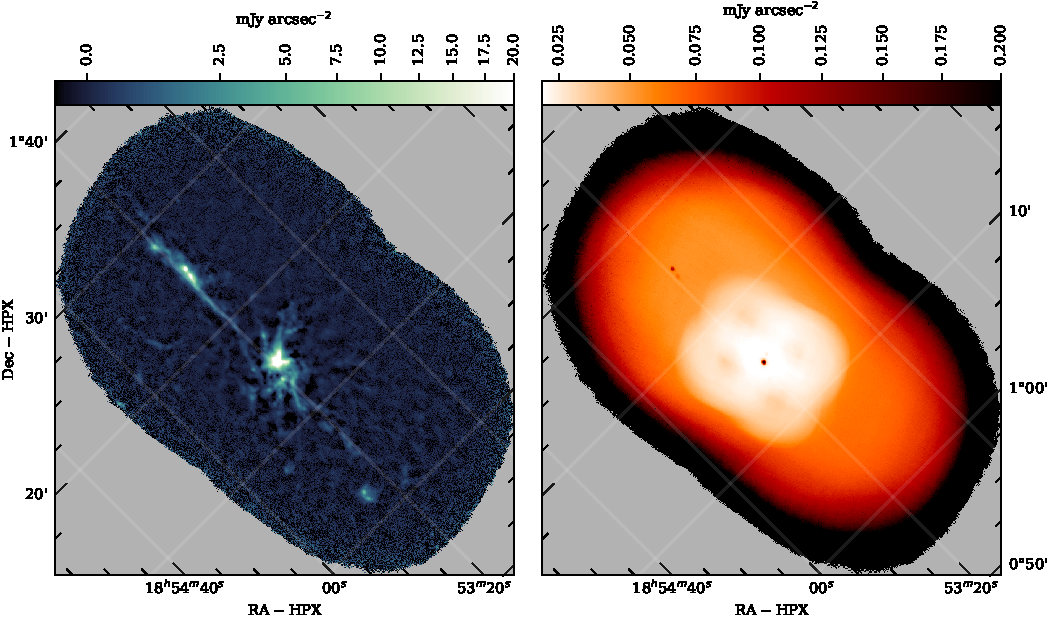
\includegraphics{tile30318-g34-coadd-noise.pdf}
  \\[3mm]
  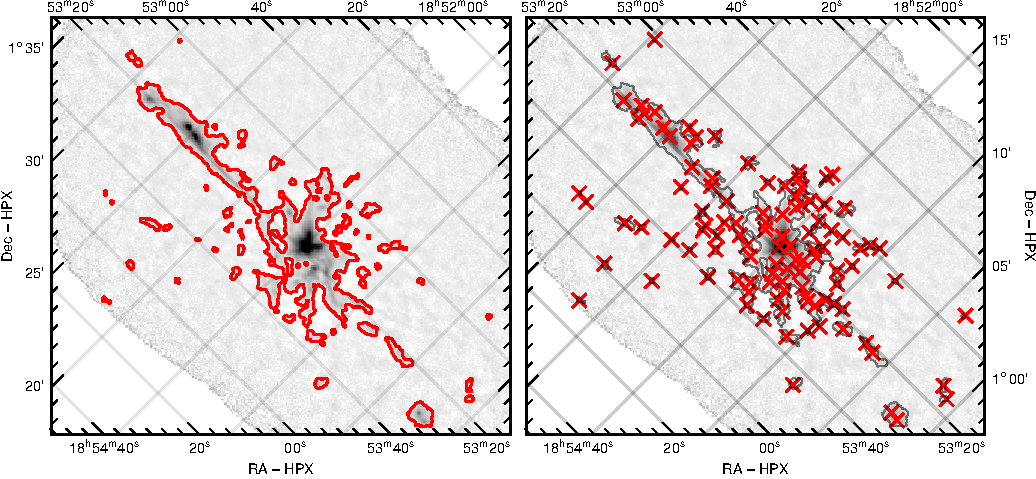
\includegraphics{tile30318-g34-extent-peak.pdf}
  \caption{The coadded products towards tile\,30318, containing the
    high-mass star-forming source G034.27+0.15. Upper left: the coadded
    emission map. Upper right: the coadded noise map, exhibiting the
    characteristic noise patterns of both the smaller DAISY
    observations in the centre, and the larger PONG observations
    around them. Lower left: the detected extents of emission,
    outlined on the coadded emission map. Lower right: the detected
    peaks within the detected extents.}
  \label{fig:g34-3}
\end{figure*}

\subsection{CRL\,618}
CRL\,618 is an extremely bright and well-studied proto-planetary
nebula, and is one of the JCMT's standard secondary flux calibration
sources for SCUBA-2. For a recent overview of it, see
e.g. \citet{Soria-Ruiz2013}. It is observed frequently with short
DAISY observations for calibration monitoring during normal nightly
science observing. As such, this coadd includes 923 observations using
51 hours of observing time across the small DAISY area, shown in
Figure~\ref{fig:crl618}. We achieved an extremely low noise due to
this large number of repeats -- achieving a noise better than
0.005\,m\jyas\ around the central source. A magnified view of the area
around the central position shows clearly a variety of point sources
detected in this deep coadd. In addition, it can readily be seen by
eye that there appear to be additional sources that are missed by our
cataloging procedure due to the negative bowling around the very
bright source. Horizontal and vertical cut throughs are shown to help
visualise this bowling.

\begin{figure*}
  \centering
  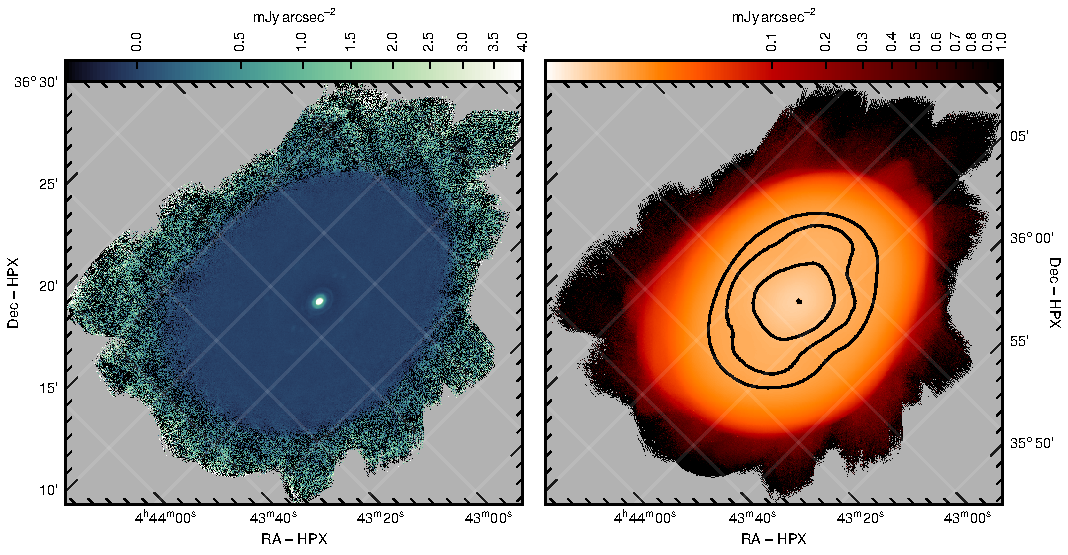
\includegraphics{crl618-whole-map.pdf}
  \\[3mm]
  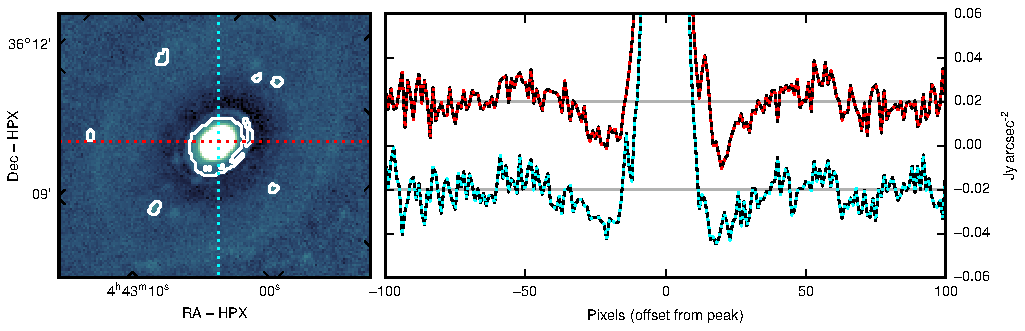
\includegraphics{crl618-sourceonly.pdf}
  \caption{Examples of the coadd, noise map, and extents towards the
    standard calibration source CRL\,618, consisting of tiles\,1238
    and 1244. This coadd contains data from 923 observations (51\,hrs
    elapsed observing time). Top left: the intensity map. Top right:
    the noise map, where the contours indicate the 0.005, 0.006, and
    0.007 m\jyas\ noise levels. Bottom left, a magnified area around
    the central source is shown with the detected extents around the
    source as white contour. Bottom right: the horizontal and vertical
    cuts through the central peak, at the positions indicated by the
    dashed lines on the bottom left plot. The upper red line has been
    offset from 0 by +0.02\,m\jyas\, and the lower cyan line by
    -0.02\,m\jyas, to allow both to be clearly seen on one plot. In
    these cuts the $\approx$ 0.02 m\jyas\ bowling around the bright
    central source can be easily seen. }
  \label{fig:crl618}
\end{figure*}

\subsection{Tile\,27258: Deep COSMOS-CANDELS field}
Here we present our deepest map. This includes data both from the JCMT
Cosmology Legacy Survey \citep[recently published by][]{Geach2016} but
also from various University of Hawai`i deep surveys
\citep{Casey2013,Chen2013,Chen2013a}. By being able to include
publicly available data taken by different projects we can achieve a
deeper map than possible with only one data set. Our coadd includes
both wide PONG observations, and very deep DAISY
observations. Figure~\ref{fig:t27258} shows both the entire tile, its
noise map, and also a close in view of the deepest region. In the noise map
it is possible to see an imprint of the original observations scan
patterns (both PONG and DAISY observations are included in this
tile); no attempt to correct for this was made. In this deep field
it can also be seen that there is no artifical structure appearing at
the edges of the different observations; this indicates that our
variance arrays (used to weight the input data at the coadding stage)
are accurate even in these high-noise areas.


In this deep map, it can clearly be seen that there are point sources
spread across the full map. Although for optimal detection of point
sources a beam matched filter should be used, even without using that
we detect a large number of these objects. Figure~\ref{fig:t27258}
shows a comparison of our detections, the CLS's detections from their
first data release \citep{Geach2016} and those of
\citet{Casey2013}. Although these three methods do not detect exactly the
same objects, there are many correspondences between them.

\begin{figure*}
  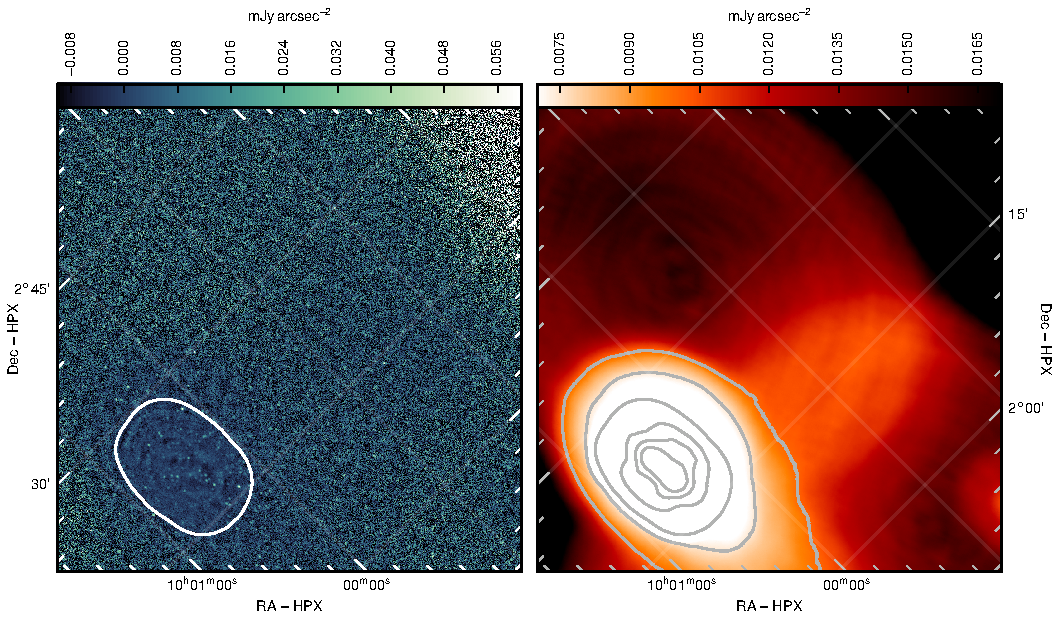
\includegraphics{27258-whole-map.pdf}
  \\[3mm]
  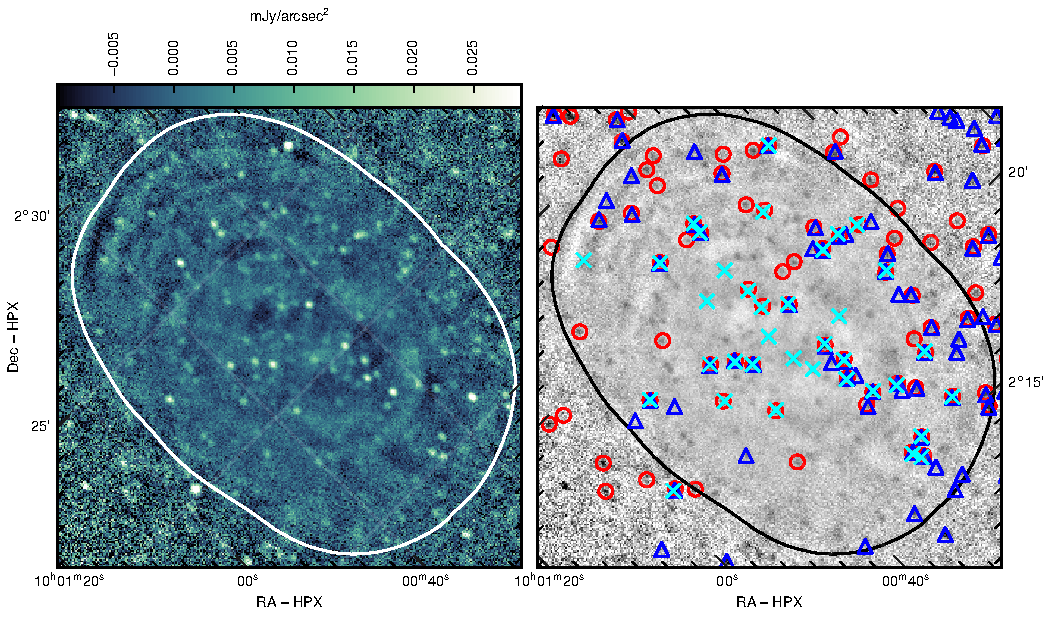
\includegraphics{27258-zoomin.pdf}
  \caption{Tile\,27258: an extremely deep coadd towards a
    COSMOS field. This tile comprises both PONG and DAISY observations
    taken by the JCMT Cosmology Legacy Survey (CLS) and several UH cosmology
    projects. Parts of these data were published in
    \citet{Casey2013,Chen2013,Chen2013a,Geach2016}. Top left: emission
    map of the entire coadded tile. A white contour indicates the
    extremely deep area with a noise < 5\,\jyas\, occurring because of
    many DAISY observations of this area.  Top right: noise map of
    the entire tile. Contours indicate the 1.75, 2, 2.5, 5, 7.5, and
    10 m\jyas\ levels. Bottom left: an enlargement of the deepest
    region of the map, showing the 850\micron\ data. The white contour
    indicates the same < 5m\jyas\ noise region. Bottom right:
    comparison of the source catalogs produced here (shown as red
    crosses), as published in \citealt{Casey2013} (black circles) and
    as found by the JCMT CLS 850um DR1 \citep[purple
    triangles]{Geach2016}, across the same enlarged region.}
  \label{fig:t27258}
\end{figure*}


\section{HEALPix grid}
\label{sec:healpix}

To produce this uniform reduction of all public data, it was necessary
to have a suitable scheme for dividing the sky into pre-determined
tiles and pixels onto which to grid the data. The scheme needed to be
well-defined in advance, without reference to the position of existing
observations, for consistency and in order to be able to easily
incorporate further data as they become public.  The tiling scheme
chosen was HEALPix \citep[Hierarchical Equal Area isoLatitude
Pixelization,][]{Gorski2005}, commonly used by cosmologists. The
HEALPix system starts by dividing the sky into twelve facets, and then
recursively divides these cells in four at each higher resolution
level.  We use the \emph{nested} numbering scheme to
label our tiles.% this scheme allows for simple conversions to and from
%positions in the HPX projection, as well as compatibility with Virtual
%Observatory systems such as MOC \citep[Multi-Order
%Coverage,][]{2013ASPC..475..135F}.

Pixels within the individual tiles use the HPX projection
\citep{Calabretta2007}, which allows us to use a (higher resolution)
HEALPix grid within our standard 2-D arrays in a FITS files. This
ensure that the pixelization is continous between each tile and the
adjacent tiles, and hence neighbouring tiles can be joined simply by
abutting them.  The details of the HEALPix parameters used are listed
in Table~\ref{tab:hpxpar}.

While HEALPix has the advantage that all pixels have the same area,
the trade off is that the pixels are not generally square: they can
vary in width and length while maintaining the constant area.  There
are also discontinuities in the angle of the grid lines at some facet
boundaries.  This is largely a display problem, as although image
viewers with a modern WCS implementation can handle files in the HPX
projection, the sources will appear distorted (or non-circular) due
the non-square pixels, and grid lines will appear bent at
discontinuities.

%\footnote{If you are concerned by
%  the visual appearance of HEALPix maps in your display and wish to
%  reassure yourself that any apparent distortion is only due to
%  display issues in your image viewer, we would recommend verifying
%  the shape and position by contouring the map over a tangent-plane
%  map.}


\begin{table}
\caption{HEALPix parameters used in this release.\label{tab:hpxpar}}
\centering
\begin{tabular}{rl}
\tableline
Tile size & $\sim$ 1\degr \\
Tile $N_\mathrm{side}$ & 64 \\
Pixels per tile  & 1024 $\times$ 1024\\
Pixel size &  $\sim$ 3.22\arcsec\\
Pixel $N_\mathrm{side}$ & $2^{16}$ \\
\tableline
\end{tabular}
\end{table}



\section{Data reduction}
\label{sec:dr}
SCUBA-2 observations are reduced using the Starlink SMURF program
\texttt{makemap} \citep{Chapin2013}. In brief, this software uses an
iterative process that divides the raw data into models of various
instrumental and astronomical signals.  For full details on the
SCUBA-2 map maker and its modelled, see \citet{Chapin2013}, or for
practical information on using the software and the effect of
different configurations in practice, see Starlink Cookbook 21
\citet{SC21}. A detailed comparison between the configuration used
here and the Gould Belt Survey reduction (tuned to recover larger
scale emission), see \citet{Mairs2015}.

%Redraft this paragraph -- more paper-esque.

There is an extremely large number of user-adjustable parameters that
can affect the final map, depending on the science goals of the users
and the structure of the astronomical emission observed.%  For example,
% a cosmologist interested in detecting only faint point sources in a
% primarily blank map would use a distinctly different set of parameters
% from a galactic astronomer looking at bright, extended and
% structurally complex emission.


% reword: previous existing configs weren't appropriate to be used on
% all types of emission. We developed one that was, with a prime
% considerationb being avoided 'blooms' or 'blobs' of fake emission
To guide astronomical users, the JCMT-supported Starlink software
comes with a series of standard configuration files for a variety of
common science cases.  Unfortunately, these standard configuration
files for \texttt{makemap} can produce very poor results when used on
an inappropriate observation -- for example, the standard SCUBA-2
configuration file used for calibrator observations is tuned to expect
a bright, compact source at the centre of the map. If used by mistake
on a blank field this recipe could easily create \emph{fake emission}
in the form of large bloom-like structures. Avoiding this sort of
error was the paramount consideration when selecting the configuration
parameters for this work.

The main focus in developing this \emph{legacy} configuration was on
maximising the confidence that could be placed in detection of
emission, at the expense of not attempting to recover large scale
structures ($>$200\arcsec{}).

These observations were reduced using Starlink, Starjava, and ORAC-DR
software developed between versions 2014A and 2015A. Interested
parties seeking to replicate these results can do so by using
the version of the code tagged as `2015A-legacy' in the
Starlink code repositories\footnote{
  https://github.com/Starlink/starlink,\newline
  https://github.com/Starlink/starjava, and \newline
  https://github.com/Starlink/ORAC-DR.}.

The exact configuration file used in the legacy reduction, is shown in
Appendix~\ref{app:config}, along with a more detailed description of
its effects. A few specific points we would like to highlight: We
explicitly filter out any size scales larger than 200\arcsec. We also
calculate a separate common-mode model for each subarray, and
therefore are not sensitive to any size scales smaller than a
subarray. We constrain the model of the astronomical signal (AST
model) via an auto-generated AST mask, which identifies all regions as
with a signal-to-noise ratio $>5$ (followed down to 3) as containing
astronomical signal. We set a convergence limit of either 25
iterations or having a change between iterations of only 1\% of the
noise level, whichever occurs first. Only 4\% of the science
observations did not converge within the 25 iterations; these were
still included in the coadds.






% See Appendix~\ref{app:config} for the full configuration file. Some of
% the most important details are described below:

% Our mapmaker configuration first of all performs five iterations without
% creating an astronomical model of the source. \note{Harriet\&DSB: do
%   we have a short explanation of do we do this again?}. It will then
% perform up to 20 further iterations with all the models, but will exit
% before that point if the 'maptol' parameter has reached a mean value
% of 0.01.

% In order to decrease the production of fake 'blooms' of emission in
% the final map, we produce a separate COMMON mode model for each
% subarray (\texttt{com.perarray=1}). While this produces more reliable
% output (appropriate for this project which has comparatively minimal
% by eye checking of data), it has the effect of removing structure
% scales that are larger than the subarray size.

% \note{zero snr and zero snrlo: need a proper explanation for these}
% We also set the 'AST' and 'FLT' zero\_snr and zero\_snrlo values.

%Figure ?? shows a reduction of a single
%observation towards a standard calibrator, reduced using both the
%legacy configuration file presented here (in an HPX projection), and
%with the standard calibration reduction configuration `bright compact'
%on the tangent plane projection.

% \begin{figure}
%   \centering
%   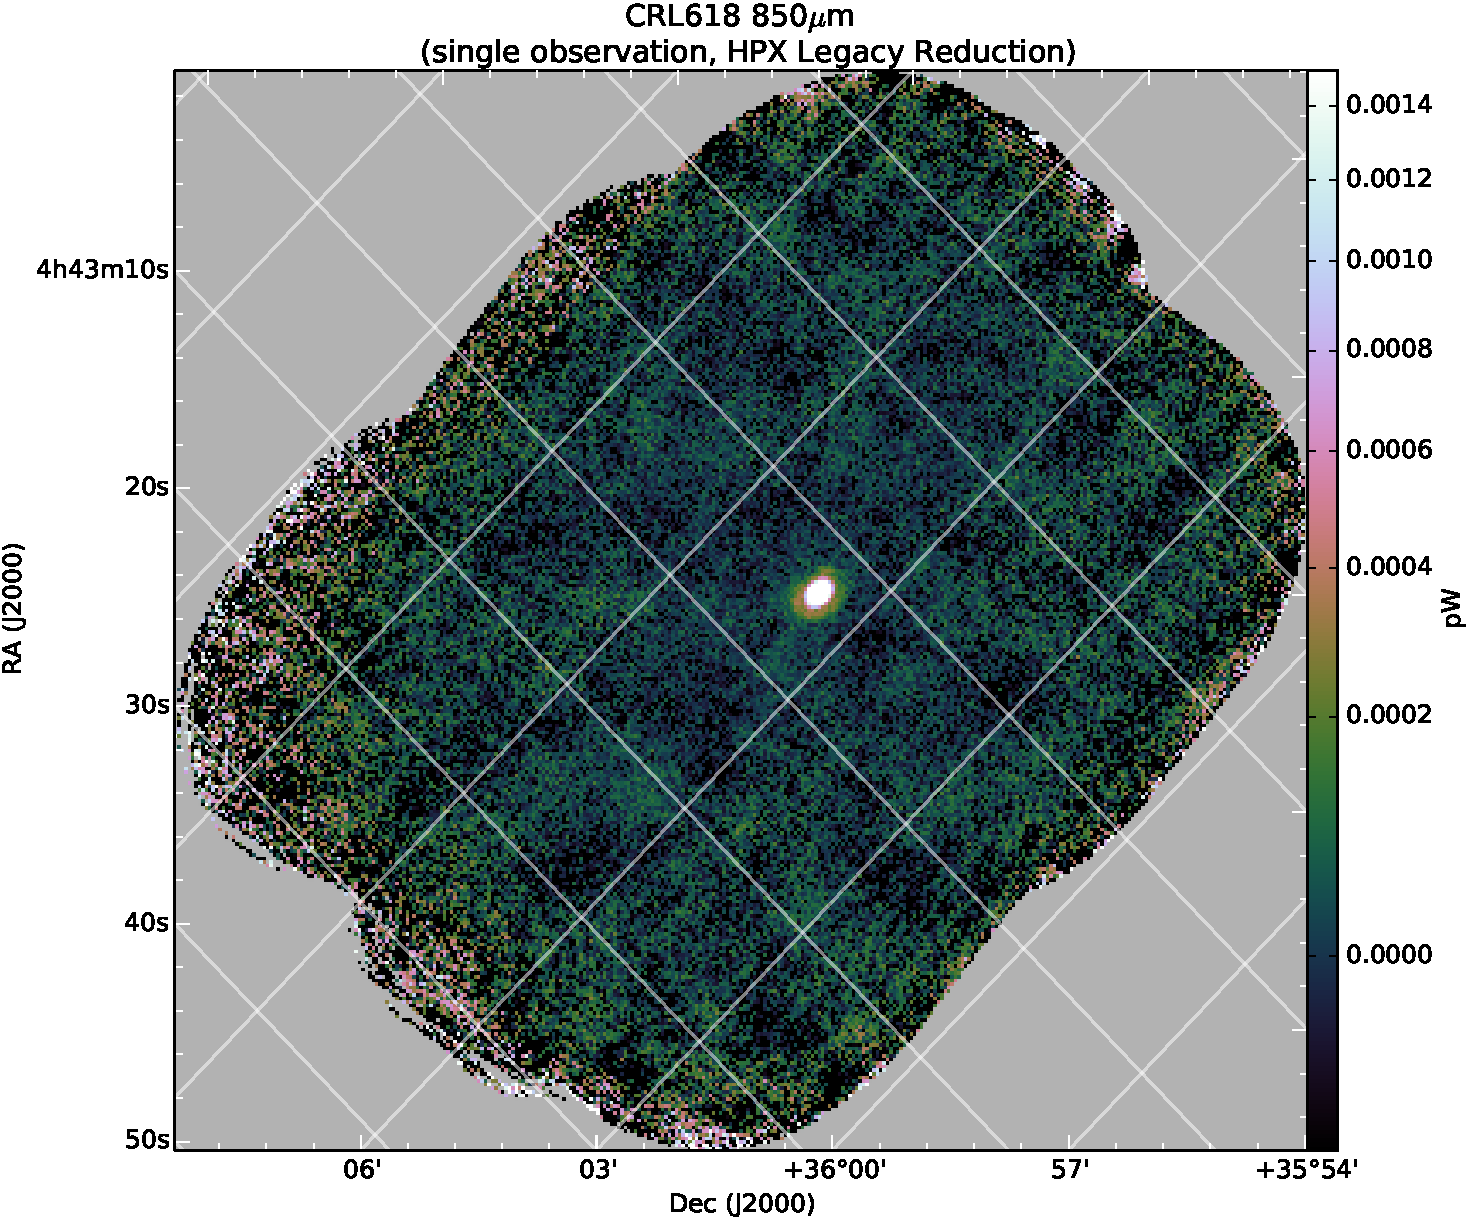
\includegraphics[width=0.45\linewidth]{crl618_example_legacyred}
%   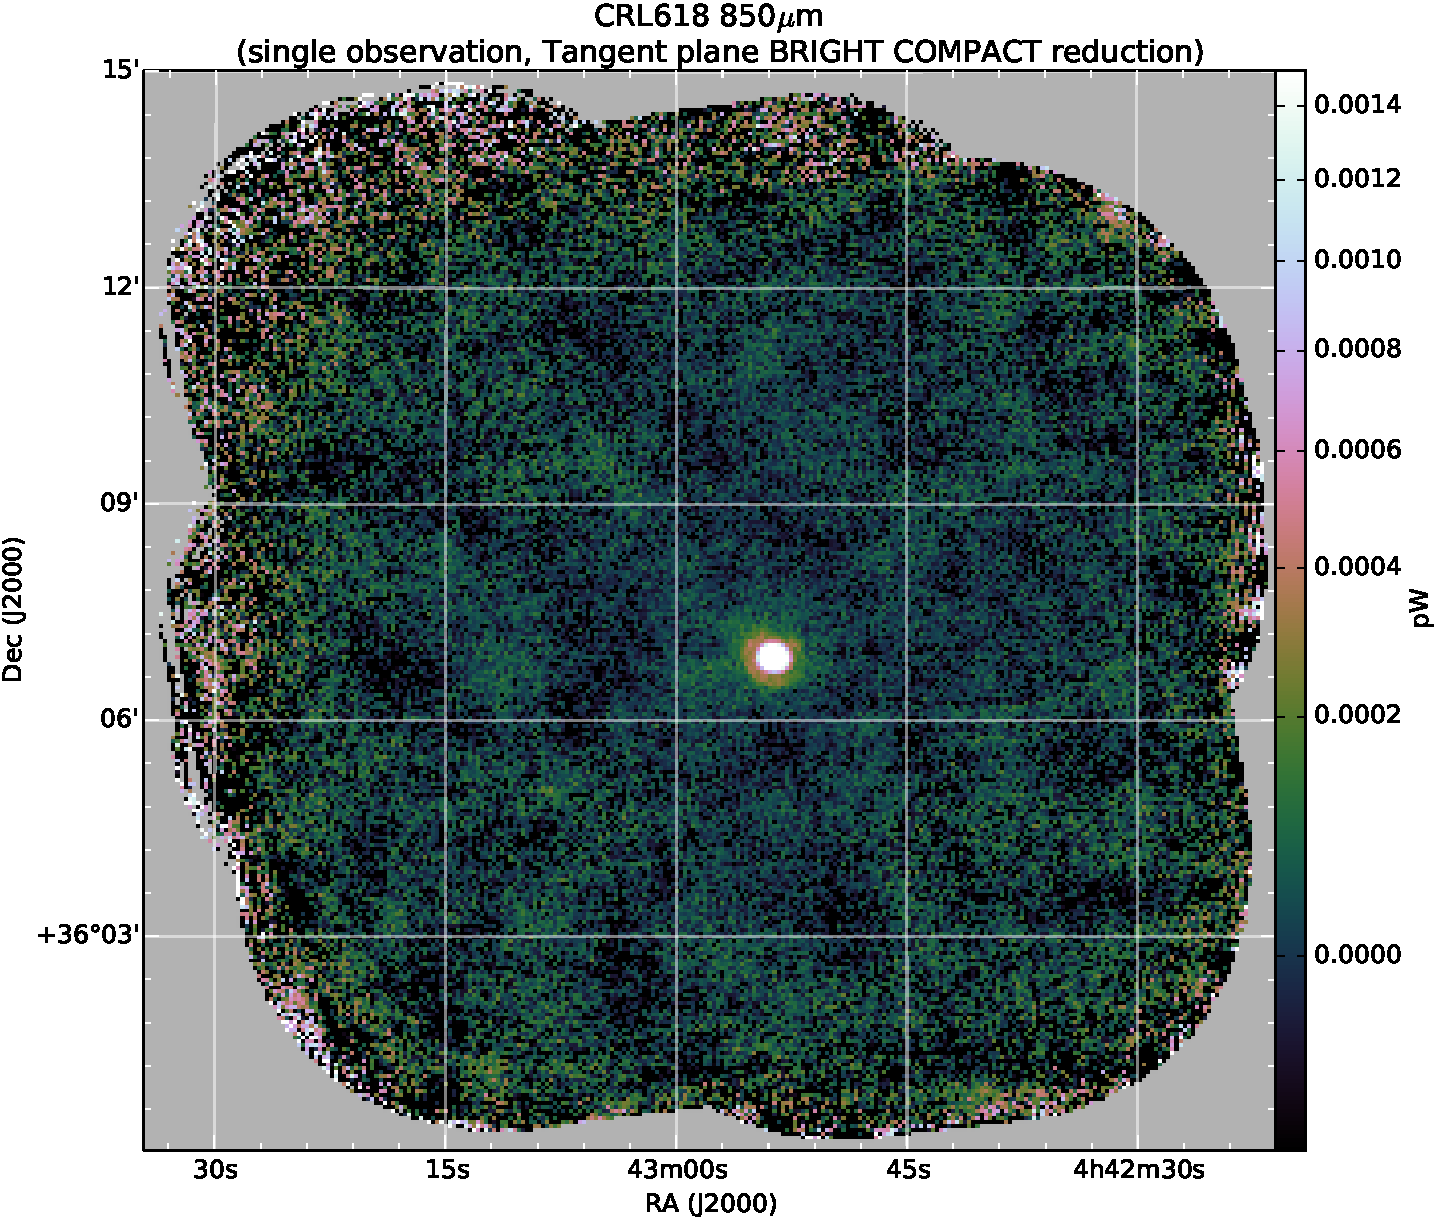
\includegraphics[width=0.45\linewidth]{crl618_example_bcred}
%   \caption{Left: A legacy 850\,\um{} reduction of a single observation
%     towards the JCMT standard calibration source CRL\,618. Note that
%     the pixel axes are at 45 degrees to the RA and Dec axes. As each
%     pixel in the map is truly shaped like a diamond (i.e. a stretched
%     square), the distortion introduced by an image viewer that
%     displays every pixel as a square causes the source to appear
%     ellipsoidal. Right: For comparison, a standard non-HEALPix tangent
%     plane reduction with the Bright Compact configuration is shown for
%     the same source. Here the source appears more circular. Both maps
%     are shown in uncalibrated units of pW on the same scale. These
%     maps cover two tiles.}
%   \label{fig:crl618-example}
% \end{figure}


%Figure ?? shows a reduction of a single
%observation towards the complex, bright, and extended OMC-1
%region. \todo{ Should this have a comparison with e.g. a GBS
%  reduction of this region, to show the difference in size scales?
%Or leave that for later}.

% \begin{figure}
%   \centering
%   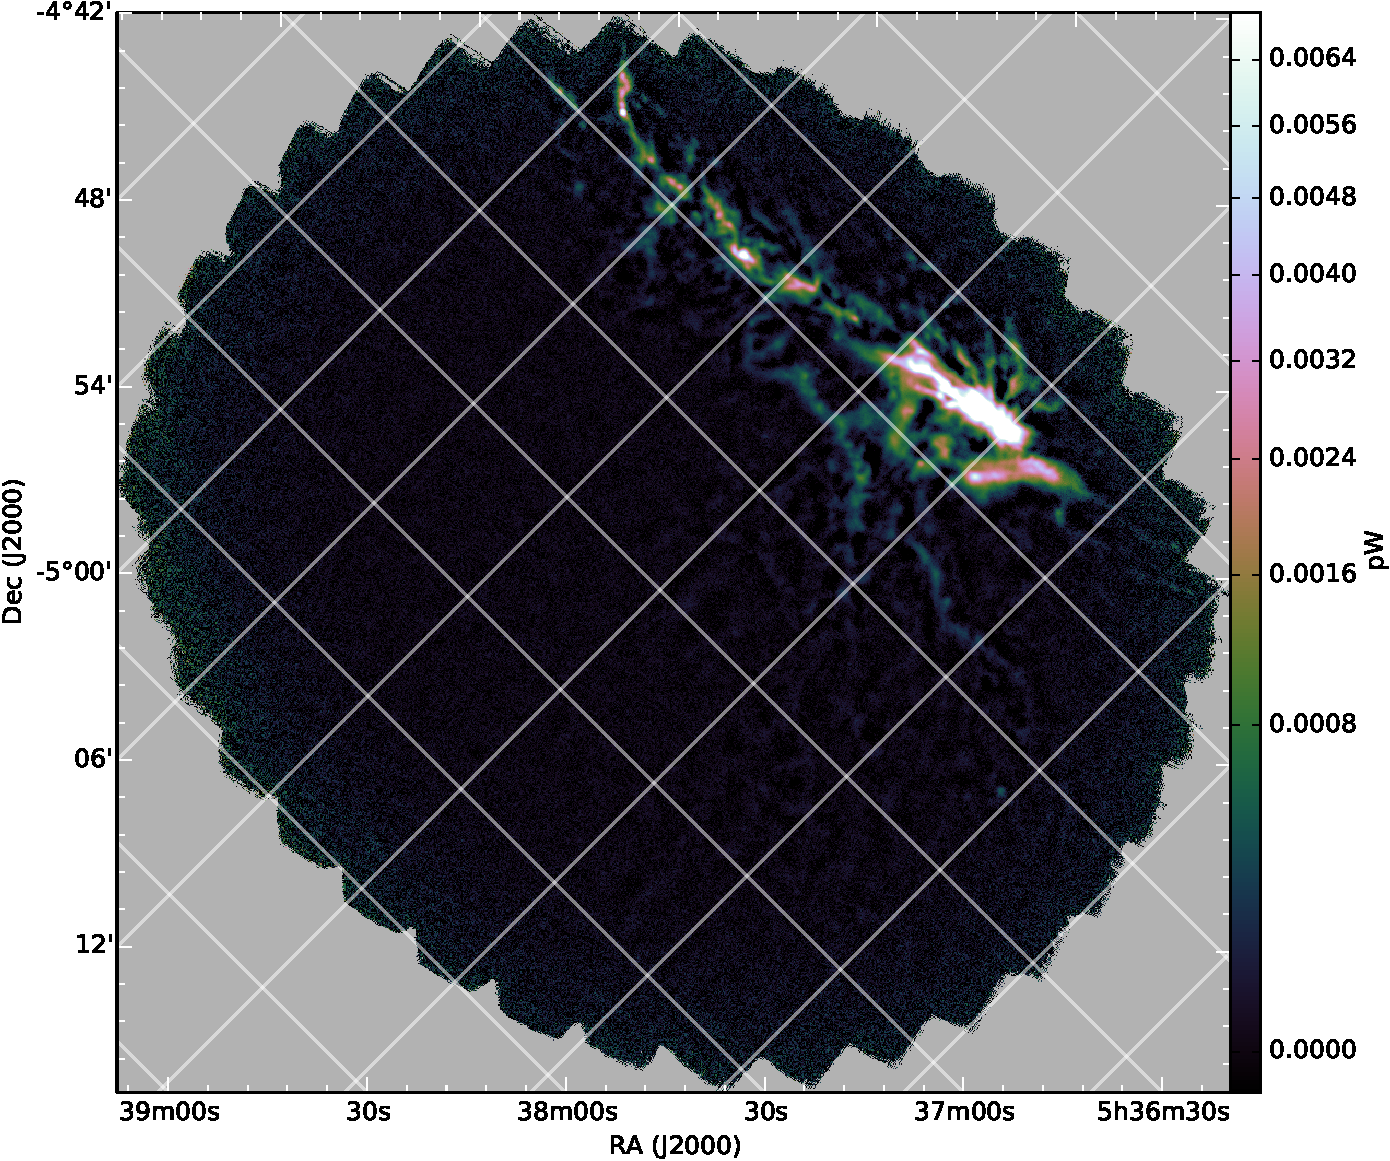
\includegraphics[width=0.6\linewidth]{omc1_example_legacy}
%   \caption{A legacy 850\,\um{} reduction of a single
%     observation(observation 93 from 2012-08-17) towards the OMC-1
%     source. This observation overlapped with three tiles: 22805, 21439 and
%     21438. }
%   \label{fig:omc1-example}
%     \end{figure}


\subsection{Quality Assurance}
\label{sec:QA}

% \subsection{Standard JCMT QA States}
% All observations taken by the JCMT are classified as \status{GOOD}
% (the default), \status{BAD}, \status{QUESTIONABLE}, \status{JUNK} or
% \status{REJECTED}. We included \status{GOOD}, \status{QUESTIONABLE}
% and \status{REJECTED} data in our coadds. The \status{REJECTED} state
% is used by the JLS teams to indicate that a particular observation did
% not meet their particular QA criterion but the data are otherwise
% usable. The \status{QUESTIONABLE} state was originally designed to be
% a transient state that would be resolved into either \status{BAD} or
% \status{GOOD} after analysis, but in practical terms there was not a
% workflow to ensure this, so some observations have this flag in the
% archive.

% Usually (in the standard nightly reduction pipelines)
% \status{QUESTIONABLE} data is treated as if it is \status{BAD} for the
% purposes of coadds. However, due to our second QA stage for this
% release, we chose to include it as long as it passed our special
% legacy QA.

% \subsection{Legacy Release QA}
% %Description of process. Examples of observations we threw out.

Every reduced observation suitable for inclusion in the coadds was
assessed by eye, and not included in the coadds if was considered low
quality.
% band marked as \status{GOOD}, \status{QUESTIONABLE} or
% \status{BAD} by a member of the Legacy Reduction team. This quick
% `by-eye' assessment was done by examining an image of the reduced map,
% and if necessary following up with more detailed examination. For the
% first data release (2011 to 2013, not including the CLS), our QA
% process only created a single plot of the intensity, and it was found
% that a lot of questionable observations required either interactive
% checking of the tile, or the manual making of an SNR image. For the
% second release (observations from 2013 to 2015, and all of the CLS),
% the QA process also used an image of the SNR map for the by-eye
% process, for easier resolution of questionable
% observations. \status{BAD} observations were excluded from the coadds,
% as were observations that were flagged as \status{BAD} by the
% observatory's normal observation-based QA (usually done during a
% night's observing). \status{QUESTIONABLE} observations were examined
% further and their state was resolved.
%
% This QA process was designed to avoid: a) `blooms' or `blobs' of fake
% emission that can sometimes be produced at the edges of the map by the
% mapmaker; and b) to identify the most problematic observations that
% had missed being flagged under the telescope standard QA process
%
% This sort of process is (of course) subjective, and some of the
% observations that we excluded might be usable on further
% examination. However, as with all of this process, the focus for this
% release has been to ensure a high-quality release, even at the expense
% of completeness.
All of these legacy-reduced observations are publicly
available through the JSA, regardless of our QA analysis of them, so
interested users can individual evaluate each observations towards a
tile if they are dissatisfied with the coadd in the release.


\subsection{Coadding of tiles}
\label{sec:coadd}
All non-pointing observations for a given tile that passed QA were
coadded and calibrated using the PICARD recipe
\texttt{COADD\_JSA\_TILES}. PICARD is part of ORAC-DR, and performs
pipeline tasks on reduced data products. This recipe uses the
\texttt{makemos} routine from Starlink's \texttt{ccdpack} package
\citep[][\ascl{1403.021}]{SUN139}. This coadding was carried out as a
variance-weighted mean. No despiking was performed, and no clipping of
the noisy edges of observations was done; no evidence was seen that
these procedures were required. The variance map for the coadded tile
was also produced. The calibration from pW into m\jyas\ was done by
multiplying by a Flux Conversion Factor of
2.46$\times$10\textsuperscript{3}\,m\jyas\,pW\textsuperscript{$-$1},
derived from our own data set -- see Section \ref{sec:calib}.

\subsection{Source Recovery}
Recently, work by \citet{Mairs2015} examined the recovery of sources
found inside and outside the \texttt{makemap} AST mask (see Section
\ref{sec:dr}), specifically comparing the JCMT Gould Belt Survey's
reductions with the Legacy Release configuration described here. They
found that in coadds of SCUBA-2 reduced observations there is a
significant difference between recovery of sources inside and outside
the AST mask. Sources that are outside the AST-masked regions can have
their flux considerably under-represented. The AST masked region in a
single observation can be thought of as approximately the region
containing detectable emission in that observation, using `detection'
limits set by the specific configuration parameters chosen. The effect
is dependent on the size of the source -- extended sources outside of
the masked regions are poorly recovered in this reduction, whereas
point sources are better recovered.  This issue does (in theory)
affect all \texttt{makemap} reductions, including those using external
masks defined from previous knowledge of the emission. However, it is
more problematic for reductions such as these, in which the AST mask
is defined based only on detected emission from a single observation.

In case users of this release are concerned about the recovery of
specific sources, each individual reduced observation contains a bit
mask (stored in a FITS extension labeled QUALITY), indicating which
areas of the map were and were not included in the AST and FLT masks.


\subsection{Size Scales}
We have excluded sizes scales larger than the subarray size from our
reduction. In addition, we have used a fairly aggressive large-scale
filtering removing scales larger than 200 arcseconds. Interested
readers are directed to \citet{Mairs2015}, which shows some examples
of the same data reduced with the JCMT Gould Belt Survey's reduction
(tuned to recover large scale structure) and with the JCMT-LR
configuration.


\subsection{Negative Bowling}
Within the coadded maps of this release, negative bowling can be
clearly seen around bright sources. Figure~\ref{fig:crl618} shows this
around the bright calibrator CRL\,618. The cuts in the vertical and
horizontal direction through the source show the bowling at
$\approx$0.02\,m\jyas.. As the size scales of the negative bowling are
comparatively large compared with small compact/point sources, this
could in theory be corrected for on a per-field basis. For this
release, no processing was done to try and ameliorate these effects,
and there will, as a result, be loss of detected emission, and the
omission of entire sources from our catalogs.


%\todo{Do we need more examples of this? Find a good description of why
%  this happens, should be in S2 cookbook somewhere.}

% \section{Comparison with legacy surveys}

% \todo{A SCUBA-2 image from each survey alongside a Legacy Release
%   version. Which wavelengths? SASSy only has one published field
%   \citep{MacKenzie2011}. JPS and NGLS may not have any yet. GBS has a
%   few recent papers with \citet{Rumble2015} published for Serpens.}


%\todo{Picture of a coadded tile? Both data and noise. Pick something
%with Daisy and pongs in it, as a comparison.}


%\todo{Each observation is gridded into pre-defined tiles. Are they
%  extinction corrected at that point? Unlike HARP processing
%  \citep{2015ACSISDR}, observations can be reduced independently and
%  then coadded. Extinction correction can be applied during coadding
%  phase? How well are edge-effects handled by variance weighting?}

\section{Calibration}
\label{sec:calib}


% \begin{itemize}
% \item show images the standard calibrators.
% \item comparison with `standard' calibrator reductions
% %\item effect of pixel size on fluxes. Per, Jess \& Daniel may have
% %  something. Doug J. and GBS did an analysis on this as well.
% \item effect of pointing errors on fluxes.?
% \item PICTURES: calibrators, comparison with bright compact and 1
%   arcsec. Examples of the coadded deep maps of all of our
%   calibrators?.
% \item Beam shape?
% \end{itemize}

The calibration of these data follows (with some changes) the basic
approach used in the standard SCUBA-2 calibration paper
\citep{Dempsey2013}. In brief, a Flux Conversion Factor (FCF) is
derived from observations of standard calibrators of known
brightnesses, which is then used to convert from the instrumental
units of pW into astronomical units. \citet{Dempsey2013} derived an
aperture FCF based on the flux within a fixed-radius aperture around
the source peak to convert into mJy\,arcsec$^{-2}$ and a beam FCF
based on a fit to the peak flux in the source, used to convert into
mJy\,beam.

For this work, we have chosen to follow \citet{Dempsey2013} and derive
both an aperture and a beam FCF. However, we have calibrated all of
our maps only using the aperture FCF as this is more appropriate for the
extraction of flux in our catalogs of detected emission.  An average
FCF was derived for the standard calibration observations taken in our
time period and reduced with the legacy configuration described above.
The reductions of each observation were left in the instrumental pW
units, and the FCF correction was applied to the coadded tiles to
produce units of mJy\,arcsec$^{-2}$. For more information about FCFs
and their derivation, please see \citet{Dempsey2013}.

Three commonly used SCUBA-2 calibrators were analysed when deriving an
FCF for this data set. These are Uranus, CRL\,618, and CRL\,2688. The
Uranus calibration observations are not part of the standard legacy
release themselves, as observations of moving targets were not
included in this release.

\citet{Dempsey2013} used a source aperture radius of 30\arcsec{} and a
background annulus of radii 45--60\arcsec. They note in their analysis
that this chosen source aperture excluded approximately 8 percent of
the Uranus flux, and provided a lookup-table of correction factors
(for use when performing aperture photometry with a different source
radius), derived from analysis of the curve-of-growth of a deep Uranus
coadd. We followed their approach by creating deep coadded maps of
our three calibration sources and analysing their curve of growth
(shown in Fig.~\ref{fig:cog}) to select appropriate source and
aperture radii. It should be emphasized that the data reduction method
used in the original paper was tuned for bright, isolated point
sources and forces a flattening of the map at radii larger than
60\arcsec, which is not done as part of our more-general-purpose data
reduction method. Based on these plots, we selected a source radius of
60\arcsec\ (chosen by eye to avoid much of the negative bowling seen around
CRL 618 and CRL 2688, while not missing too much of the flux from
Uranus, which extends out further), and a background annulus from
105-120\arcsec\ (chosen to avoid the ringing structure detected in the
deep coadds).

\begin{figure}
  \centering
  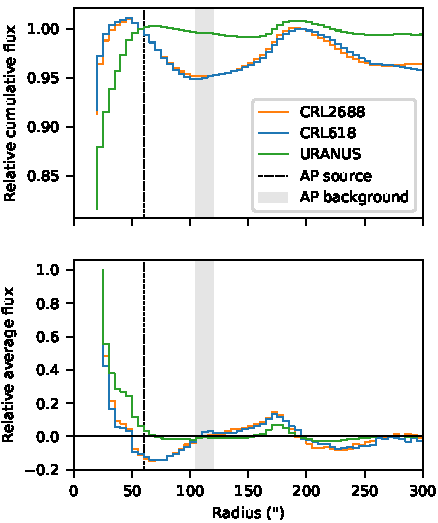
\includegraphics{cog-relative60arcs.pdf}
  \caption{The curve-of-growth for the deep coadded maps of Uranus,
    CRL\,618 and CRL\,2688. The top plot shows all flux included
    within a radius of the given size, normalised to the flux for that
    source in an aperture of 60" radius. The bottom plot shows the
    average flux per pixel in an annulus at the given radii,
    normalised to the flux in the first annulus. The 60\arcsec\ radius
    and the 105-120\arcsec background annulus used in the aperture
    photometry(AP) FCF derivation are indicated on the plot.}
  \label{fig:cog}
\end{figure}



Using these apertures, an aperture FCF was then derived for the
JCMT-LR 850\,\micron\ reduction of each calibration observation
towards these three sources.\footnote{CRL 618 and CRL 2688
  observations that had been marked as poor quality during QA were not
  included in this analysis.}  The Uranus observations from the time
period covered by this release had been separately reduced using the
same SCUBA-2 configuration and pixel size, but not onto a HEALPix grid
as Uranus is a moving target. The maps were masked with the
appropriate circles/annulus and the source and background statistics
were calculated using the ATOOLS and KAPPA Starlink
packages.\footnote{The \texttt{autoastrom} command does not account
  for non-square pixels, so was not used for this analysis.}  The
KAPPA command \texttt{beamfit} was also used to fit the amplitude of
the beam, and this was used to calculate the beam FCF. The Starlink
FLUXES package \citet{2014ascl.soft05010J} was used to derived the
expected flux of Uranus at the time of each observation. For CRL\,618
and CRL\,2688, the integrated and peak fluxes measured in
\citet{Dempsey2013} were used.
\begin{equation}
  \label{eq:1}
  \mathrm{FCF_{arcsec}} = \frac{S_{\mathrm{integ}}}{I_{0}A}\ \mathrm{Jy\,pW^{-1}\,arcsec^{-2}}
\end{equation}

\begin{equation}
  \label{eq:2}
  \mathrm{FCF_{beam}} = \frac{S_{\mathrm{peak}}}{I_{\mathrm{peak}}}\ \mathrm{Jy\,pW^{-1}\,beam^{-1}}
\end{equation}

Where $S_{integ}$ is the known integrated flux in the source and
$S_{peak}$ is the known peak flux in the source (both from FLUXES for
Uranus, or from \citet{Dempsey2013}), $I_{0}$ is the summed flux in
the aperture of the map (minus the flux in the background annulus),
$I_{peak}$ is the peak amplitude of the BEAMFIT Gaussian fit to the
map, and $A$ is the area of a pixel in the map
($3.22^2\,\textrm{arcsec}^{2}$). The histograms of the derived FCFs
are shown in Figure \ref{fig:fcfhist}

\begin{figure}
  \centering
  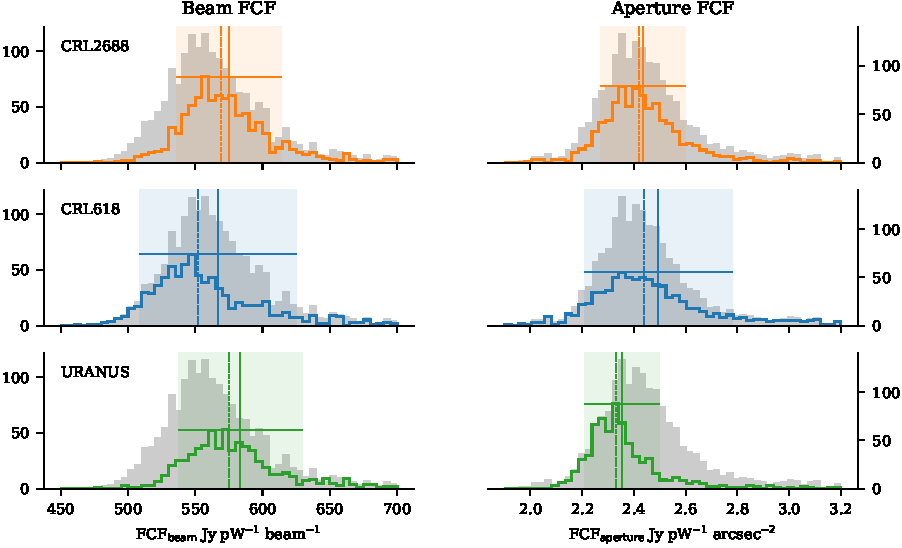
\includegraphics{fcf-histogram.pdf}
  \caption{Histograms of the derived beam and arcsecond FCFs
    separately for CRL618, CRL2688 and Uranus. The combined histogram
    for CRL 618 and CRL2688 (i.e. the sources used to derive the
    calibration of the coadds) is shown as a grey background. The
    sigma-clipped mean for each source is shown as the vertical line,
    and the horizontal cross bar indicates the $\pm$ one standard
    deviation.}
  \label{fig:fcfhist}
\end{figure}


\subsection{Effect of AST masking on derived FCF}

The recovery of source emission in SCUBA-2 observations reduced with
\texttt{makemap} is strongly dependent on the exact details of the AST
mask, unless the reduction configuration does not use one. \citet{Mairs2015} looked
in some detail at a comparison between the recovery in flux of sources
inside and outside the AST mask, for the LR \texttt{makemap}
configuration. They found from simulations that the flux in sources
outside the mask is suppressed compared with the 'true' value, and
compared with sources inside the mask. In this reduction we use an
auto-generated AST mask that finds sources with a 5-$\sigma$ detection
at each iteration (and follows them down to a 3-$\sigma$ limit); this
means that our AST mask, and hence flux recovery, is dependent on the
brightness of the sources and the noise in the observation.


This has an important, but often ignored, effect on the flux recovery
and derived FCFs from our calibration observations: very bright
sources, such as Uranus, will have a larger area included in the AST
mask due to a higher signal-to-noise at a given RMS, when compared
with dimmer sources such as CRL\,618 and CRL\,2688. We believe this
variation in the AST model size causes the very different curves of
growth for Uranus as opposed to CRL\,618 and CRL\,2688 (see Figure
\ref{fig:cog}). We believe this is also responsible for the difference
in the arcsecond FCF mean values for Uranus (see \ref{fig:fcfhist}) --
not a dramatic difference with the 60\arcsec\ source aperture used
here, but more obvious at some aperture sizes.  For reference, Uranus
has an integrated flux between 57.2 and 70.3 Jy for the observations
in this analysis (from FLUXES), whereas CRL\,618 has a flux of 5.0 Jy,
and CRl\,2688 has a similar flux of 6.13\,Jy \citep[both
from][]{Dempsey2013}.

% The issue occurs due to the effect of the automatic AST masking used
% in the data reduction, combined with the extreme variation in the
% source brightnesses. In our configuration, an AST mask is produced
% each iteration around every source with an SNR peak greater than 5,
% and followed down to include all connecting pixels with an SNR greater
% than 3. If we compare the three calibration sources Uranus, CRL 618,
% and CRL 2688, these sources have significantly different
% brightnesses. CRL\,618 has an integrated flux of 5.0 Jy, CRL\,2688 is
% 6.13 Jy, whereas Uranus varies between 57.2 and 70.3 Jy for the
% observations in this analysis.

Therefore, for an observation reaching a similar noise level in the
map, the auto-generated AST mask will have a different size for each
source (based on their brightness -- see Figure
\ref{fig:astmask}). This will then cause different proportions of the
flux in the source to be recovered in the final map, due to the
differing recovery in \texttt{makemap} reductions of flux within and
without the beam.

As a result, when performing aperture photometry at a specific source
aperture, different proportions of the `true' total source flux will
be found for sources of different brightnesses. This will cause a
measurable difference in the measured FCF for the sources when using a
constant aperture. In particular, Uranus observations have a much
larger AST mask, and thus will have a higher proportion of their total
integrated flux found at a specific aperture. This leads to a
derivation of a smaller FCF for Uranus than for the dimmer calibration
sources.

This effect would not be seen in the `canonical' analysis presented in
\citet{Dempsey2013}, as the \texttt{makemap} \texttt{bright\_compact}
configuration used there sets a fixed AST aperture with a radius
of 60\arcsec\ for all sources, constraining all pixels beyond this
radius to zero until the last iteration.


To illustrate this problem visually, we have simulated 50 point
sources at various peak brightnesses (in pW) from 0.002 pW to 0.1 pW,
and reduced them using the \texttt{jsa\_generic} configuration. This
roughly ranges from a quarter of the peak intensity of CRL\,618 (which
has an average peak brightness of 0.009 pW in these observations)
to roughly the brightness of Uranus (an average peak of 0.11
pW). These maps were created using the \texttt{fakemap} and
\texttt{fakescale} options to \texttt{makemap}, with a source model
taken from the central 200$\times$200 pixel square found in a deep coadd of
800 Uranus observations, and using a single blank DAISY observation
for the SCUBA-2 data. Figure~\ref{fig:simulation} shows the variation
in source brightness and relative derived FCF for a variety of
different source and background apertures. For reference,
Figure~\ref{fig:astmask} shows the relationship between the area of
the AST mask with the brightness of the simulated source.

\begin{figure}
  \centering
  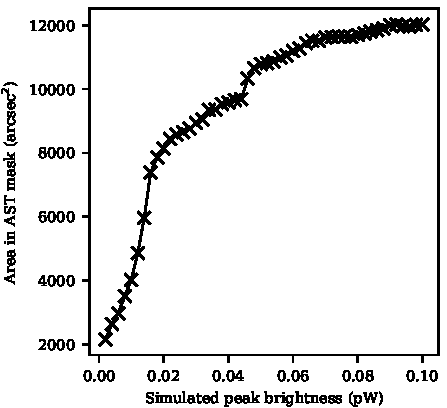
\includegraphics{astmask-peakbrightness.pdf}
  \caption{The relationship between the area of the AST mask and the
    brightness of the simulated source. The AST mask area is found
    by counting the number of pixels included in the final AST mask,
    and multiplying by the area of one pixel.}
  \label{fig:astmask}
\end{figure}


\begin{figure}
  \centering
  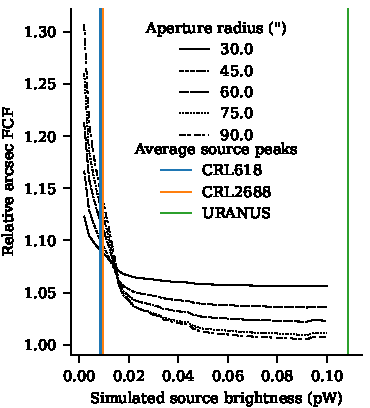
\includegraphics{simulated-fcfs.pdf}
  \caption{Simulated FCFs derived for 50 simulated point sources with
    peak brightnesses from 0.002--0.1\,pW, and using various aperture
    radii. The average peak brightness of our three calibration
    sources are indicated on the map. The input source was derived
    from a deep coadd of Uranus. The background map was a blank
    850\,\um\ DAISY observation.}
  \label{fig:simulation}
\end{figure}

% plot of relative FCF for simulated bright source at various apertures and brightnesses

% plot of area included in AST mask at different brightnesses

% plot of relative FCF vs area in AST mask.
\subsubsection{Effect of transmission}
Due to the signal-to-noise limits in the AST masking, there will also
be a similar systematic effect in the measured FCF of a calibration
due to the RMS noise in the observation. Higher-noise observations
will have a smaller area in their SNR-defined AST mask, and thus a
higher FCF will be calculated. As the major determiner of the noise is
the 850\,\um\ transmission of the observation, this will lead to a
variation in derived FCF with both weather and elevation. Figure
\ref{fig:fcfairmass} shows the derived arcsecond FCFs plotted against
the 850\,\um\ transmission. A slight trend can clearly be seen. For
comparison, we also give the variation in derived arcsecond FCFs with
time. No correction to the FCF for sky opacity or date was made in
this release.

\begin{figure}
  \centering
  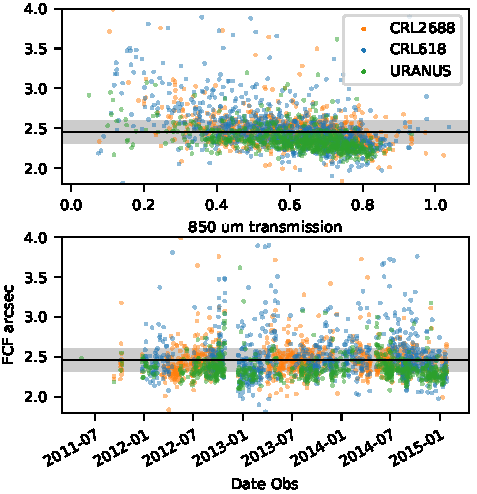
\includegraphics{fcf-extra.pdf}
  \caption{The variation of arcsecond FCFs with 850\,\um\ transmission
    (top) and with time (bottom). The arcsecond FCF used to calibrate
    this release, and its standard deviation, are shown at the solid
    black line and surrounding gray area. A clear (slight) trend can
    be seen between FCF and the transmission of the observation. Some
    extreme outliers have been cropped from the plots.}
  \label{fig:fcfairmass}
\end{figure}



%\hl{Please note that there is an additional complication here, in that the
%autogenerated AST mask actually varies in area \emph{at each
%  iteration}.}

\subsection{Derivation of mean FCF}
%plot of histogram of 850um fluxes

Despite the larger systematic uncertainty from the AST masking
effects, we have chosen here for simplicity and consistency to
calibrate this data release using a single aperture FCF. As Uranus
is far brighter than anything in our released observations, we have
chosen to only use CRL\,618 and CRL\,2688 to derive our FCF value. We
used the derived FCF from each calibration observation described
above, then applied an iterative clipping which excludes FCF values
5-$\sigma$ away from the mean (as extreme outliers will often be due
to poor instrumental performance, bad weather, daytime observing or
other affects that are not present in the bulk of the released data.)
No explicit cut was made for the atmospheric transmission during the
calibrator observations, as no cut was made to the science
observations included in the coadds. Figure \ref{fig:fcfhist} shows
histograms of the full distributions for each source.  The final
average values found are:

\begin{eqnarray}
\mathrm{FCF}_{\mathrm{arcsec},850}&=&2.46 \pm 0.22\ \mathrm{Jy}\ \mathrm{pW}^{-1}\  \mathrm{arcsec}^{-2}.\\
\mathrm{FCF}_{\mathrm{beam},850}&=&571 \pm 48\ \mathrm{Jy}\ \mathrm{pW}^{-1}\ \mathrm{beam}^{-1}.
\end{eqnarray}

% \begin{figure}
%   \centering
%   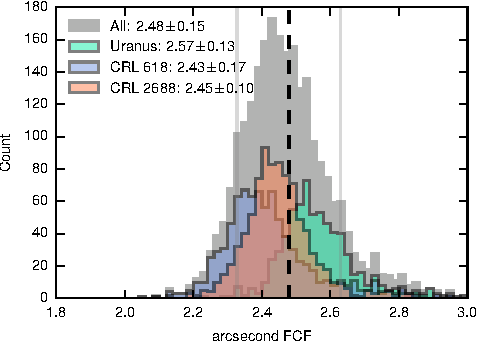
\includegraphics{lrvalues-histo}
%   \caption{Histogram of FCFs, both for all sources (light gray) and
%     separately for each source. The derived average FCF is shown as
%     the dashed vertical line, with the $\pm$1s.d. shown as the light
%     gray lines to either side.}
%   \label{fig:calibhist}
% \end{figure}

The coadds in this release were calibrated using this mean arcsecond
FCF.  This standard deviation represents a 1-$\sigma$ uncertainty of
approximately 9 percent. All coadds were calibrated using the same
FCF. If subsequently a user of this release wishes to use a different
FCF calibration value, they can divide the coadded maps or catalogue
fluxes by our standard FCF, and then recalibrate by multiplying with
their chosen FCF.


The standard deviation of the sample of derived FCFs represents the
minimum uncertainty in this calibration. In addition, the standard
error in the sub-mm flux of Uranus should also be taken into
account. \citet{Dempsey2013} quote this as $\pm$ 5 percent. Taken
together in quadrature, this gives an overall estimated uncertainty in
calibrated fluxes of $\pm$10 percent due only to the variation of
these derived FCFs.

For comparison, the usual `canonical' 850\,\micron\ arcsecond FCF used
in the JCMT's nightly reductions is $2.34 \pm 0.08 \mathrm{Jy}\
\mathrm{pW}^{-1}\ \mathrm{arcsec}^{-2}$ \citep{Dempsey2013}. This is
approximately 3 percent lower than the value used here, and was
derived using the `bright compact' \texttt{makemap} configuration on 1
arcsecond pixels (in comparison with the 3.22$\times$3.22 arcsecond
pixels in this release), using observations taken from 2011 May to
2012 May.

% Don't care that much about comparison with the legacy FCF?

%Fig.\,\ref{fig:lr-caldb-histo} shows the comparison between the
%histograms of bright compact derived FCFs and the legacy release
%derived histogram, for the same
%observations. Fig.\,\ref{fig:lr-caldb-scatter} shows the scatter plot
%of each bright compact FCF vs the legacy release FCF for each
%observation. Broadly speaking, we see an approximately linear
%relationship between the two derivations of FCF.

% \begin{figure}
% 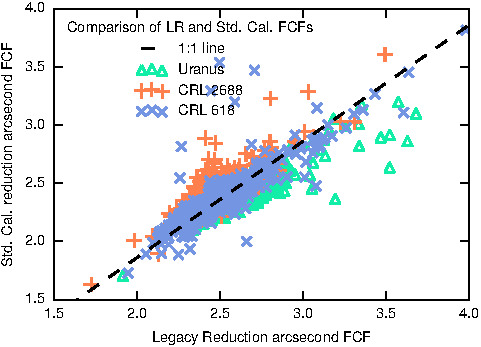
\includegraphics{legacyFCF-caldbFCF-scatter.pdf}
% \caption{Comparison between the FCFs derived from the legacy release
%   reductions, and those derived from the standard JCMT SCUBA-2
%   calibrator reduction. The dashed line indicates a one-to-one
%   relationship, offset by the difference in the derived FCF used for
%   calibrating the legacy release (2.48) and the canonical FCF (2.34)
%   from \citet{Dempsey2013}. \label{fig:lr-caldb-scatter} }
% \end{figure}

%To show the variation seen in the individual FCFs, we provide for
%reference plots of the histogram of the FCFs
%(Fig.~\ref{fig:calibhist}), the variation in FCF with opacity
%(Fig.~\ref{fig:calibvstrans}) and the variation in FCF with date
%(Fig.~\ref{fig:calibvstime}). No correction to the FCF for sky opacity or date
%was made in this release.

% \begin{figure}
% 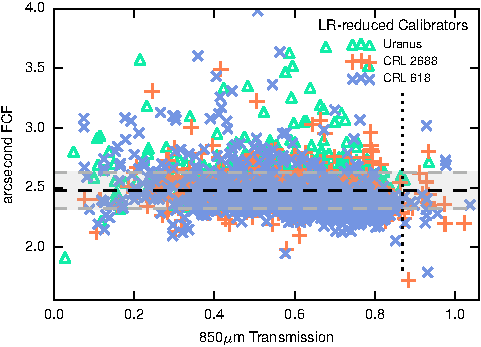
\includegraphics{legacyFCF-vs-transmission.pdf}
% \caption{The legacy arcsecond FCFs derived from CRL\,618, CRL\,2688 and
%   Uranus, shown against the 850\micron\ atmospheric transmission
%   during the observation. Horizontal lines indicate the derived mean
%   and standard deviation of the FCFs.\label{fig:calibvstrans}}
% \end{figure}

% \subsection{Effect of AST masking on the source calibration}
% As can be seen from figure\ref{fig:calibhist}, we appear to see
% different distributions of derived arcsecond FCFs for Uranus as
% compared with CRL 618 \& CRL 2668. We believe this is due to the
% difference in brightnesses in the source, when combined with the AST
% masks produced in the reductions. In our configuration, an AST mask is
% produced each iteration around every source with an SNR peak greater
% than 5, and followed down to include all connecting pixels with an SNR
% greater than 3.

% The recovery of source emission in SCUBA-2 observations reduced with
% \texttt{makemap} is strongly dependent on the exact details of the AST
% mask used in the reduction (unless an AST model is not used). See
% e.g. Mairs et al 2016 for detailed discussion of this effect when
% comparing the brightness of sources found inside and outside the AST
% region. However, as well as the effect on faint sources found outside
% the AST mask, it is important to note that the AST model will also
% have an effect on our derivation of arcsecond Flux Calibration Factors
% using aperture photometry.

% If we compare the three calibration sources Uranus, CRL 618, and CRL
% 2688, these sources have significantly different brightnesses. This
% means that for an observation reaching a similar noise level in the
% map, the auto-generated 3-sigma AST mask will include differing areas
% of the map for each source (based on their brightness). This will then
% cause different proportions of the flux in the source to be recovered
% in the final map, due to the differing recovery in \texttt{makemap}
% reductions of flux within and without the beam.

% %(You could consider this difference in area as almost corresponding to
% %probing a different proportion of the JCMT/SCUBA-2 beam, in an
% %observation of the same noise level.)



% Therefore, when performing aperture photometry at a specific source
% aperture, different proportions of the `true' total source flux will
% be found for sources of different brightnesses. Effectively, this will
% cause a measurable difference in the FCF for the sources. In
% particular, Uranus (ranging in brightness between 57 and 70 Jy) will have
% a larger AST mask, and thus will have a higher proportion of its
% 'true' integrated flux found at a specific aperture. This will lead to
% a derivation of a smaller FCF for Uranus than for the dimmer
% calibration sources.

% This affect would not be seen in the `canonical' analysis presented
% in Dempsey et al 2013, as the \texttt{bright\_compact} configuration in
% that analysis uses  a fixed AST aperture with a radius of 60\arcsec\ for all
% sources, constraining all pixels beyond this radius to zero until the
% last iteration.

% To help visualise this effect, we present in in
% Figure \ref{fig:astmasks} a comparison of the areas included in the AST
% masks found by source. It can be seen that the AST mask for Uranus, by
% far the brightest source, covers a significantly larger area than that
% of the CRL 618 and CRL 2688 sources.

% To illustrate this further, we have simulated a set of point sources
% at various brightnesses (in pW) from 0.002 pW to 0.1 pW, and reduced
% them using the \texttt{jsa\_generic} configuration. These maps were
% created using the \texttt{fakemap} and \texttt{fakescale} options to
% \texttt{makemap}, with a source model taken from the central 200x200
% pixel square found in a deep coadd of 800 Uranus observations, and
% using a single blank Daisy observation for the SCUBA-2
% data. Figure~\ref{fig:simulation} shows the variation in source
% brightness and relative derived FCF for a variety of different source
% and background apertures.


% Please note that there is an additional complication here, in that the
% autogenerated AST mask actually varies in area \emph{at each iteration}.

\subsection{Additional uncertainties in the final flux values}

\citet{Dempsey2013} derived appropriate FCFs for either point sources
or for circular aperture photometry, and we have followed their
approach here. However, it is clear that for the arbitrary shaped
regions of emission found in the catalogs of this release, it would
not be appropriate to perform circular aperture photometry. As
discussed above, this would also not be sufficient to correct for the
different proportions of flux included inside the AST mask.

As such, we present the integrated and peak flux found within our
sources, calibrated using the arcsecond FCF derived for CRL 618 and
CRL 2688 using aperture photometry, without attempting to correct for
these effects or subtract any backgrounds. In practice, it should be
assumed that there is an additional significant (and not completely
known) uncertainty on fluxes presented here, or indeed on any flux
found by simple integration of flux found within an arbitrary
shape. From our analysis of simulations of point sources above, it is
likely that there are systematic trends where lower flux is more
poorly recovered than brighter flux. If highly accurate fluxes are
required, it may be necessary to perform detailed simulations
investigating the total flux recovery for a given AST mask. We would
also recommend users of this release interested in this to
investigate the AST mask found for the individual observations
that went into each mosaiced tile.


\section{Catalogs}
\label{sec:cat}
The JCMT Legacy Release includes emission catalogs generated from each
of the coadded maps. As we have an extremely diverse set of
astronomical regions (including blank fields, point sources, and large,
complex extended structures), we did not feel that it would be
possible to perform specific astronomical source finding and
classification within the scope of this release. Instead, we
first of all identified the \emph{regions of contiguous
  emission}, discussed here as \emph{extents}, and secondly identified
\emph{local maxima within those regions}, described here
as \emph{peaks}. The primary goal of these catalogs is to provide
astronomers with regions of securely detected emission.


We have chosen to use the FellWalker algorithm \citep{Berry2015}, as
implemented in the Starlink \texttt{cupid} \citep{cupid} package for this
analysis. Unlike the more commonly used ClumpFind, which simply lays
discrete contour levels on the map and uses those to identify regions,
FellWalker follows lines of ascent within the map to identify all
peaks of emission. We have found it to be robust and
easy-to-understand.

\subsection{Extents}
\label{sec:extents}
We have identified the regions of contiguous extended emission within
each tile by looking at the signal-to-noise maps of the coadded
tiles. We chose to consider all regions of contiguous emission
containing a pixel brighter than 5-$\sigma$, followed down to a limit
of 3-$\sigma$, to be a single `extent' for the purposes of our catalogs,
if the region is larger in area than a beam.  Here, a very simple
approximation of the beam was used: all sources comprising more than
nine pixels were kept. More complex approaches were considered,
but noise spikes did not appear to be commonly falsely detected as
emission with this simpler approach. The main source of false detections in
our reductions \emph{would} have been the previously discussed problem of
`false blooms', if we had not used a by-eye approach for flagging the
handful of problematic reductions and removing them from the coadds.

The reduced observations, produced by SMURF's \texttt{makemap} routine, all
contain a variance array giving a noise estimate for each pixel, based on
the scatter of input data values to that pixel. Pixels with too few
inputs to calculate a variance point are not included in
the individual maps. Our coadding procedure uses this variance to
weight the input observations.

We used the FellWalker algorithm as implemented in \texttt{cupid} on a
signal-to-noise (SNR) map to produce contiguous regions of emission
and to identify the position of the peak pixel within each map, and
these outlines are available both as a FITS format mask file, as a
HEALPix Multi-Order Coverage file \citep{2013ASPC..475..135F}. The
catalog for each tile indicates the ID of the clump, the RA and Dec of
the peak pixel's centre, the total flux contained within the entire extent, the
flux of the peak pixel, and the area of the entire extent. The catalog
also includes the approximation of the outline of the extent as an
STC-S \citep[Space-Time Coordinate String]{2009ivoa.rept.1030R}
polygon. An excerpt from the extent catalog for tile\,30318
(containing G34.3) is shown in Table~\ref{tab:extents}.



\subsection{Peaks}
\label{sec:peaks}
In order to provide some information about the nature of emission
within the extents, this release includes identification of local
maxima within the extents. \emph{It is important to note that these
  should not in general be considered as point sources.} We identified
these maxima by running the FellWalker algorithm (from \texttt{CUPID})
on the regions we had previously identified as being in
\emph{extents}. The peak detections were not created from the SNR map,
as we could assume by only looking within the detected extents that we
were already looking at detected emission.

As our maps contain a varying noise, we adopted the mean noise across
the entire detected extent (from the variance array produced by
\texttt{makemos}) as a representative noise. We then ran the FellWalker
algorithm, using that representative noise as the RMS value, and
identified as individual local maxima all peaks  with a value of at least
5-$\sigma$, followed down to a noise level of 3-$\sigma$, and with at
least a 5-$\sigma$ dip between them and their neighboring peaks. Our
output catalog contains the ID of the peak, the RA and Dec of the peak
pixel, the flux in the peak pixel, and the ID of the extent the peak
was found within. An excerpt from the peak catalog for tile\,30318 is
shown in Table~\ref{tab:peaks}.

We chose not to include the outlines of all emission counted as
being within that object or clump, as we felt that would encourage
users to consider the peaks as being discrete physical objects. Although
they may be in some cases, in many other cases the peak is simply a
local maximum within a complex molecular cloud. The `clump outlines'
produced by algorithms such as FellWalker always reflect the arbitrarily
chosen boundaries of dips and minimum heights, and should not be
assumed to represent physical objects without considerable further
modeling.


%\footnote{To re-grid one or more HEALPix tiles onto a standard RA-Dec
%  projection, the Starlink \textsc{smurf} command \texttt{jsajoin} can
%  be used \citep[][\ascl{1310.007}]{SUN258}.}



% \section{Noise}

% % coadds contain 1.69 gigapixels of non bad data.
% %
% \begin{itemize}
% \item Noise maps: overlaps work fine, show an example?
% \item Copy COHRS pixel distribution graph?
% \item noise on each pixel, noise vs integration time.
% \item High noise towards bright sources.
% \end{itemize}




%Noise vs integration time
% this is harder to do -- how to do a scatter plot of with billions of
% points.. 2-d histogram instead? produce in same way as the noise
% coadds.

% Anomalous variance array values towards bright sources USe OMC-1 and
% CRL 618 as examples? Also visible in G34.3 shown earlier. Mentioned
% earlier.

\section{Pointing}
\label{sec:pointing}
\begin{figure}[htb!]
  \centering
  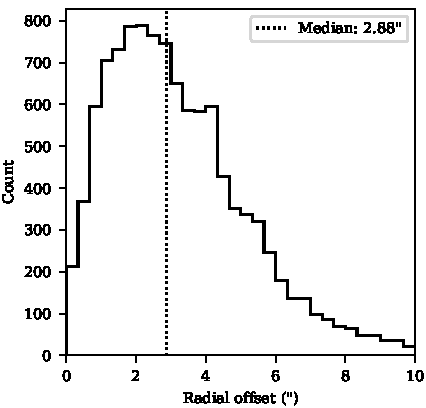
\includegraphics{pointing-offset.pdf}
  \caption{Histogram of the total magnitude of the position offsets
    found in the calibration observations (including pointings). The
    median value of 2.88\arcsec{} is indicated on the plot.}
  \label{fig:pointing}
\end{figure}

% explain the position fudging done for the calibration sources.
Our observations of JCMT standard calibrators and pointing sources are
corrected for normal pointing offsets, as these sources are all at
known positions. In our data reduction stage, these observations are
run through \texttt{makemap} twice; first to calculate the difference between
the beam position and the known source position, and secondly
re-reduced using this positional offset to place the observation at
the correct point. No other observations in this data set were
corrected for their positions.


The JCMT usually quotes a pointing offset of approximately 2\arcsec{}
in $x$ and $y$, corresponding to an average radial offset of
2.9\arcsec{}. By examining the offsets in RA and Dec found for the
calibrator and pointing observations, we identified that the average
pointing offset for the release matches this expected value, with a
median radial offset of 2.88\arcsec{}. See Figure~\ref{fig:pointing}
for the histogram of these offsets.  In general, we can assume that
the pointing in our non-calibration observations should be on average
\emph{more} accurate than this, as the JCMT operators will correct for
offsets found in a pointing observation before they continue with the
science observations. When examining coadded science observations, if
the beam area is required to a high accuracy than a correction factor
for beam smearing may need to be included.


\section{Beamshape}
\label{sec:beam}
\begin{figure*}[htb!]
  \centering
  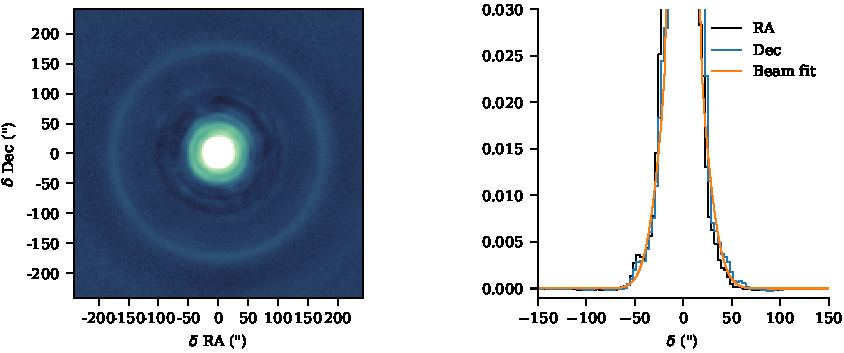
\includegraphics{beamfit-uranus.pdf}
  \caption{The SCUBA-2 850\micron\ beam, as found from a deep coadd
    of Uranus observations. On the left is shown an image of the
    central source. The bright ring at ~160" radius is due to
    misaligned panels on the telescope. On the right: profiles in RA
    and Dec of the beam are shown with the fitted two-Gaussian beam
    model overlaid for contrast. The $y$-axis shows the value relative
    to the full amplitude of the beam.}
\label{fig:beam}
\end{figure*}




Using the same deep coadded maps of Uranus as we examined in Section
\ref{sec:calib}, we fitted a two-component beam model to the JCMT
beamshape, and found the same shape and size as found in
\citet{Dempsey2013}. We use the KAPPA command \texttt{beamfit} to do
this, fitting two circular Gaussians with a fixed background level of
0. We found FWHM of 12.6\arcsec\ and 44.0\arcsec\, with a relative
amplitude of 96 percent and 4 percent. Figure \ref{fig:beam} shows the
image of the deep Uranus coadded maps, as well as a comparison
between the radial profiles along the horizontal and vertical axes and
the fitted beam shape.



\section{Accessing the Release}
The data products forming the JCMT Legacy Release are fully included
in the CADC's multi-observatory archive (which includes the JSA), and
will return as appropriate in searches based on spatial, temporal and
spectral limits. This is hosted at
\url{http://www.cadc-ccda.hia-iha.nrc-cnrc.gc.ca/en/search}

Our uncalibrated reductions of single observations can be found by all
the same criteria which would identify the raw and normal reductions
of that observation -- including telescope, proposal code, PI name,
target name, as well as the spatial, temporal and spectral
constraints.

In addition, user's can search specifically within the tiles and the
catalogs by searching for proposal ID \texttt{JCMT-LR} along with any
other desired constraints, or to see the all coadds and catalogs at
once they can go to
\url{http://www.cadc-ccda.hia-iha.nrc-cnrc.gc.ca/en/search/?Observation.proposal.id=JCMT-LR&Observation.Collection=JCMT}
Please note that you will find there are extent-850um results shown
for all tiles, even those where no emission was detected. \hl{I still
  think this may be bad idea -- who wants to see a catalog plane
  returned where there is no detection??? It would be much better to
  include the tile MOC in the coadd plane instead of in the
  extent-850um plane}


Appendix \ref{sec:filetypes} summarises what scientific content is
included in the files produced in this release, along with the
productID under which they are listed within the JSA, the naming
scheme for the file and  the software that created the file.


For convenience, we have also provided a single-file download
combining all of the extent and peak catalogs on the EAO/JCMT website
at: \url{INSERT\ URL\ HERE}.

\section{Summary}
\hl{Summarise the release and why it is amazingly awesome and useful.}


\acknowledgments
The James Clerk Maxwell Telescope has historically been operated by
the Joint Astronomy Centre on behalf of the Science and Technology
Facilities Council of the United Kingdom, the National Research
Council of Canada and the Netherlands Organisation for Scientific
Research. This work was funded by the Science and Technology
Facilities Council.  Additional funds for the construction of SCUBA-2
were provided by the Canada Foundation for Innovation.

The work presented here was initially started by the Joint Astronomy
Centre, and latterly has been supported by East Asian Observatory (EAO).
EAO has operated the JCMT since 2015 March 1, on behalf of the
National Astronomical Observatory of Japan, Academia Sinica Institute
of Astronomy and Astrophysics, the Korea Astronomy and Space Science
Institute, the National Astronomical Observatories of China and the
Chinese Academy of Sciences (Grant No. XDB09000000), with additional
funding support from the Science and Technology Facilities Council of
the United Kingdom and participating universities in the United
Kingdom and Canada.

This research used the facilities of the Canadian Astronomy Data
Centre operated by the National Research Council of Canada with the
support of the Canadian Space Agency. Many thanks are due to the staff
of CADC for their help with various technical aspects of this release.

The authors wish to recognize and acknowledge the very significant
cultural role and reverence that the summit of Maunakea has always had
within the indigenous Hawaiian community.  We are most fortunate to
have the opportunity to conduct observations from this mountain.

 \vspace{5mm}
\facility{JCMT(SCUBA-2)}

% Comma separated list, include software citations here as \citep{}
% after name of software, before next comma.
\software{Starlink \citep{2014ASPC..485..391C,2011ascl.soft10012V},
  SMURF \citep{2013ascl.soft10007J},
  SMURF-makemap \citep{Chapin2013},
  KAPPA \citep{2014ascl.soft03022C},
  ORAC-DR \citep{2015oracdr,2013ascl.soft10001J},
  ATOOLS,
  CCDPACK \citep{2014ascl.soft03021W},
  CUPID \citep{2013ascl.soft11007B},
  FLUXES \citep{2014ascl.soft05010J},
  Astropy \citep{2013A&A...558A..33A}, % units, fits, tables, wcsaxes
  Healpy \url{https://github.com/healpy},
  PyMOC \url{https://github.com/grahambell/pymoc}
}

\bibliography{legacy-850um-paper}
\bibstyle{aasjournal.bst}




\clearpage
\appendix


\section{Mapmaker configuration}
\label{app:config}
The mapmaker configuration used for this release (known as a
\texttt{dimmconfig} file) is shown here. Like most SCUBA-2 mapmaker
configuration files, it first includes the \emph{base}
\texttt{dimmconfig} file that sets up the basic values for a range of
options and then tweaks a subset of parameters for its
purposes. This file is included in the 2015A Starlink release. The
value of every configuration parameter used is written into the
history component of the reduced file.

\begin{verbatim}
^$STARLINK_DIR/share/smurf/dimmconfig.lis

#  Less aggressive cleaning to cope with bright sources
noisecliphigh=10.0
dcthresh = 100

#  Don't want extended structure, so avoid problems with COM model by using
#  individual common-mode models for each subarray.
com.perarray = 1

#  Aggressive filtering.
flt.filt_edge_largescale=200

#  Allow bolometer noise to vary with time, and using a box filter to
#  determine mean noise in each box, in order to presevre as many samples
#  as possible.
noi.box_size=-15
noi.box_type=1

#  Use a maximum of 20 iterations
numiter=-25
maptol_mean=1
maptol=0.01

# new recommendations and using an ast model
ast.zero_snr = 5
ast.zero_snrlo = 3

ast.skip=5
flt.zero_snr=5
flt.zero_snrlo=3
\end{verbatim}



\subsection{Details of the legacy DR configuration}
In this particular reduction, after the initial pre-processing stage,
the SCUBA-2 mapmaker recipe performs five iterations in which the
astronomical model (AST) is retained at the end rather than being
removed as in a normal iteration. (This is specified using
\texttt{ast.skip=5}). These initial iterations allow the reduction
process to focus on creating a mask for the FLT model (which is used
to filter the low frequency noise) by identifying any unusually bright
region; these regions may cause ringing in subsequent estimates of the
low-frequency noise in each bolometer. During these iterations
``bright'' pixels are taken to be those with a signal-to-noise ratio
greater than 5.0, plus any other pixels that are attached contiguously
to such pixels down to an SNR of 3 (specified by using
\texttt{flt.zero\_snr=5} and \texttt{flt.zero\_snrlo=3}).

During each iteration, an atmospheric opacity correction is applied
and the data are filtered to remove any features on scales larger than
200\arcsec. In addition to this, a separate common-mode model is
produced for each subarray (specified with
\texttt{com.perarray=1}). Having a separate common-mode estimate per
subarray prevents artificial flux (also known as ``fake blooms'')
being introduced into the map where the common modes vary
significantly and are not well represented by a single common
mode. The disadvantage with having a separate common mode for each
subarray is that the reduction is limited to recovering emission
structures that are on the same scale or less than the subarray size
(approximately 200").

After the initial five iterations, the recipe then performs up to 20
further iterations with all the models (specified by
\texttt{numiter=-25}; the initial five iterations plus these
additional 20 iterations containing all models). The number of total
iterations was limited to 25 so that time to reduce all observations
in this release was not excessive. Each of these remaining iterations
removes the AST model of the astronomical signal from the residuals
prior to starting the next iteration. However, to prevent
instabilities in the iterative process, this subtraction only occurs
within regions corresponding to bright sources.  The AST mask
identifying such sources is created in the same way as the mask used
by the FLT model: source pixels are taken to be those with a
signal-to-noise ratio greater than 5.0 (plus any other pixels that are
attached contiguously to such pixels down to an SNR of 3 (specified by
using \texttt{ast.zero\_snr=5} and \texttt{ast.zero\_snrlo=3}).  The
map maker exits before the 20th iteration if the \texttt{maptol}
parameter -- the change between maps -- has reached a mean value of
1\% of the noise level (specified by \texttt{maptol=0.01}) Only 562 of
the science observations (4.4 percent) did not converge within the 25
iterations. These were not flagged and were included in the coadded
tiles.

\newpage
\section{Full listing of file types in this release}
\label{sec:filetypes}
\movetabledown=2in
\begin{rotatetable}
\begin{deluxetable}{llp{4.5cm}p{3.5cm}p{3.5cm}l}
%\tabletypesize{\scriptsize}
\tablewidth{\linewidth}

\tablecolumns{7}
\tablecaption{Listing of all types files contained in this data release.}
\tablehead{\colhead{Object} & \colhead{recipe} & \colhead{filename} & \colhead{Contained in file} & \colhead{Notes} & \colhead{productID}}
\startdata
Single observation
& \multicolumn{1}{p{2.5cm}}{REDUCE\_SCAN\_JSA\_PUBLIC}
& \texttt{jcmts<YYYYMMDD>\_<SCAN>\_850\_healpix<TILE>_obs_000.fits}&
\raggedright{\textbullet{} Emission map (pW)}\linebreak
\raggedright{\textbullet{} Variance map (pW\textsuperscript{2})}\linebreak
\raggedright{\textbullet{} Quality map (bit mask)}
& Multiple files per observation, one for each tile the observation fell onto & healpix-850um\\
%
Coadded tile &  COADD\_JSA\_TILES  & \texttt{jcmts850um\_healpix<TILE>\_pub\_002.fits} &
\raggedright{\textbullet{} Emission map (m\jyas)}\linebreak
\raggedright{\textbullet{} Variance map (m\jyas)\textsuperscript{2}}
 & One file per tile & healpix-850um\\
%
Extent catalog & JSA\_CATALOGUE&\texttt{jcmts850um\_extent-cat<TILE>\_pub\_002.fits}
&\textbullet{} Catalog for extents (see Sect.\,\ref{sec:extents})
& Only created if  emission detected at $>5\sigma$. & extent-850um\\
%
Extent mask & JSA\_CATALOGUE & \texttt{jcmts850um_extent-mask<TILE>\_pub\_002.fits} &
\textbullet{} Mask map indicating which pixels fell into which extent
& " & "\\
%
Extent MOC & JSA\_CATALOGUE & \texttt{jcmts850um\_extent-moc<TILE>\_pub\_002.fits} &
\textbullet{} MOC file, indicating which pixels fell into any extent & " & "\\
Peak catalog & JSA\_CATALOGUE & \texttt{jcmts850um\_peak-cat<TILE>\_pub\_002.fits} &
\textbullet{} Catalog of peaks (see Sec.\,\ref{sec:peaks})&
Only created if extents catalog created. & peak-850um\\
%
Coverage MOC & JSA\_CATALOGUE & \texttt{jcmts850um\_tile-moc<TILE>\_pub\_002.fits} &
\textbullet{} MOC file, identifying all pixels that contain valid data (as opposed to blank pixels) & Created for all tiles. & extent-850um\\
\enddata
\tablecomments{In the filename column, \texttt{<SCAN>} indicates the
  JCMT scan number of that observation, padded with zeros to five-digit
  length. \texttt{<YYYYMMDD>} indicates the UT date of the
  observation. \texttt{<TILE>} indicates the HEALPix tile number of
  that tile, using the nested scheme and the HEALPix parameters given
  in Table\,\ref{tab:hpxpar} ($N_\mathrm{side}$ = 64).
  \\
  The \emph{single observation} files will be found in the JSA under the
  original observation's metadata, observation ID, and project code. All
  remaining files are in the JSA in a tile-centric fashion, and are found under the project
  code `JCMT-LR', with metadata appropriate for the specific tile, and
  with an observation ID of the form \texttt{SCUBA-2-<TILE>}.}
\end{deluxetable}
\end{rotatetable}
\newpage
\section{Example Catalogs}
Excerpts from the extent and peak catalogs of tile\,30318.
\movetabledown=2in
\begin{rotatetable}
\begin{deluxetable}{c c c c c c p{7cm}}
\tablecaption{An excerpt from the catalog of extents for Tile 30318.\label{tab:extents}}
\tablehead{\colhead{ID} & \colhead{RA} & \colhead{DEC} & \colhead{TOTAL_FLUX} & \colhead{PEAK_FLUX} & \colhead{AREA} & \colhead{SHAPE}\\ \colhead{ } & \colhead{deg} & \colhead{deg} & \colhead{$\mathrm{mJy}$} & \colhead{mJy\,arcsec$^{-2}$} & \colhead{arcsec$^{-2}$} & \colhead{ }}
\startdata
JCMTPX_J185318.8+011459 & 283.3285 & 1.2497 & 5.415E+09 & 2.105E+02 & 1.633E+05 & Polygon ICRS TOPOCENTER 283.3003 1.256714 283.2408 1.289357 283.3113 1.273799 283.3003 1.308009 283.3347 1.306843 283.3283 1.386135 283.3019 1.392549 283.3381 1.488935 283.3406 1.306847 283.3964 1.189091 283.3532 1.215324 283.3594 1.166936 283.3271 1.152366 283.339 1.196665 283.2928 1.201333 \\
JCMTPX_J185334.7+011421 & 283.3944 & 1.2392 & 2.599E+06 & 1.647E+00 & 8.609E+03 & Polygon ICRS TOPOCENTER 283.3889 1.235147 283.3855 1.240392 283.3759 1.241558 283.3841 1.256706 283.3878 1.257872 283.391 1.268366 283.3944 1.268947 283.3958 1.260787 283.4051 1.254378 283.3996 1.246216 283.4026 1.238634 283.4102 1.231055 283.4109 1.222318 283.4074 1.221737 283.4061 1.226401 \\
JCMTPX_J185330.0+010240 & 283.3752 & 1.0445 & 5.236E+06 & 5.745E+00 & 7.148E+03 & Polygon ICRS TOPOCENTER 283.3608 1.032857 283.3603 1.036351 283.3624 1.039264 283.3612 1.04218 283.3621 1.049172 283.369 1.051884 283.3841 1.050334 283.3866 1.046261 283.3845 1.039849 283.3871 1.035768 283.3848 1.034608 283.382 1.029943 283.3738 1.023732 283.3669 1.029947 283.3635 1.030529 \\
JCMTPX_J185322.6+010831 & 283.3443 & 1.1419 & 2.774E+05 & 9.040E-01 & 2.702E+03 & Polygon ICRS TOPOCENTER 283.3363 1.137201 283.3392 1.141282 283.3408 1.148856 283.3491 1.15235 283.3518 1.150022 283.3523 1.147694 283.347 1.13429 283.3436 1.131768 283.3367 1.135266 \\
JCMTPX_J185321.5+010610 & 283.3395 & 1.1028 & 7.271E+05 & 1.185E+00 & 4.310E+03 & Polygon ICRS TOPOCENTER 283.3337 1.100475 283.3335 1.105721 283.3351 1.109802 283.3321 1.117381 283.3367 1.122421 283.3388 1.121457 283.339 1.117381 283.3461 1.102807 283.3468 1.098726 283.3447 1.094645 283.3472 1.088237 283.3381 1.083192 283.3347 1.085322 283.3347 1.088812 283.3392 1.09348
\enddata
\end{deluxetable}

\end{rotatetable}
\begin{deluxetable}{ccccc}
\tablecaption{An excerpt from the catalog of peaks for Tile 30318.\label{tab:peaks}}
\tablehead{\colhead{ID} & \colhead{RA} & \colhead{DEC} & \colhead{PEAK_FLUX} & \colhead{PARENT_EXTENT}\\ \colhead{ } & \colhead{deg} & \colhead{deg} & \colhead{mJy\,arcsec$^{-2}$} & \colhead{ }}
\startdata
JCMTPP_J185318.8+011459 & 283.3285 & 1.2497 & 2.105E+02 & JCMTPX_J185318.8+011459 \\
JCMTPP_J185318.2+012524 & 283.3257 & 1.4234 & 4.608E+01 & JCMTPX_J185318.8+011459 \\
JCMTPP_J185316.0+011518 & 283.3168 & 1.2550 & 3.018E+01 & JCMTPX_J185318.8+011459 \\
JCMTPP_J185318.7+012445 & 283.3278 & 1.4124 & 2.470E+01 & JCMTPX_J185318.8+011459 \\
JCMTPP_J185316.5+011434 & 283.3189 & 1.2427 & 2.004E+01 & JCMTPX_J185318.8+011459 \\
JCMTPP_J185321.6+011341 & 283.3401 & 1.2281 & 1.224E+01 & JCMTPX_J185318.8+011459 \\
JCMTPP_J185320.8+012825 & 283.3367 & 1.4736 & 7.523E+00 & JCMTPX_J185318.8+011459 \\
JCMTPP_J185319.8+011257 & 283.3326 & 1.2159 & 5.712E+00 & JCMTPX_J185318.8+011459 \\
JCMTPP_J185315.2+011713 & 283.3134 & 1.2870 & 4.566E+00 & JCMTPX_J185318.8+011459 \\
JCMTPP_J185318.2+011339 & 283.3257 & 1.2276 & 2.932E+00 & JCMTPX_J185318.8+011459 \\
JCMTPP_J185316.9+011318 & 283.3202 & 1.2217 & 2.896E+00 & JCMTPX_J185318.8+011459 \\
JCMTPP_J185328.2+011350 & 283.3676 & 1.2305 & 2.699E+00 & JCMTPX_J185318.8+011459 \\
JCMTPP_J185322.5+011211 & 283.3436 & 1.2031 & 2.474E+00 & JCMTPX_J185318.8+011459 \\
JCMTPP_J185326.9+011251 & 283.3621 & 1.2142 & 2.456E+00 & JCMTPX_J185318.8+011459 \\
JCMTPP_J185323.4+011137 & 283.3477 & 1.1937 & 2.224E+00 & JCMTPX_J185318.8+011459 \\
JCMTPP_J185324.3+011119 & 283.3511 & 1.1885 & 2.164E+00 & JCMTPX_J185318.8+011459 \\
JCMTPP_J185320.5+012224 & 283.3353 & 1.3733 & 2.119E+00 & JCMTPX_J185318.8+011459 \\
JCMTPP_J185307.1+011600 & 283.2797 & 1.2666 & 2.098E+00 & JCMTPX_J185318.8+011459 \\
JCMTPP_J185318.2+012722 & 283.3257 & 1.4561 & 2.053E+00 & JCMTPX_J185318.8+011459 \\
JCMTPP_J185326.9+011551 & 283.3621 & 1.2643 & 1.935E+00 & JCMTPX_J185318.8+011459 \\
JCMTPP_J185325.4+011318 & 283.3559 & 1.2217 & 1.769E+00 & JCMTPX_J185318.8+011459 \\
JCMTPP_J185319.2+012653 & 283.3298 & 1.4479 & 1.654E+00 & JCMTPX_J185318.8+011459 \\
JCMTPP_J185311.4+011617 & 283.2976 & 1.2713 & 1.638E+00 & JCMTPX_J185318.8+011459 \\
JCMTPP_J185316.7+012629 & 283.3195 & 1.4415 & 1.546E+00 & JCMTPX_J185318.8+011459 \\
JCMTPP_J185323.8+011047 & 283.3491 & 1.1798 & 1.528E+00 & JCMTPX_J185318.8+011459 \\
JCMTPP_J185316.7+011638 & 283.3195 & 1.2771 & 1.292E+00 & JCMTPX_J185318.8+011459 \\
JCMTPP_J185305.3+011549 & 283.2722 & 1.2637 & 1.278E+00 & JCMTPX_J185318.8+011459 \\
JCMTPP_J185320.5+012043 & 283.3353 & 1.3453 & 1.212E+00 & JCMTPX_J185318.8+011459 \\
JCMTPP_J185318.2+011623 & 283.3257 & 1.2730 & 1.204E+00 & JCMTPX_J185318.8+011459 \\
JCMTPP_J185320.3+011921 & 283.3347 & 1.3226 & 1.091E+00 & JCMTPX_J185318.8+011459 \\
JCMTPP_J185325.9+011407 & 283.3580 & 1.2351 & 9.760E-01 & JCMTPX_J185318.8+011459 \\
JCMTPP_J185321.5+012657 & 283.3395 & 1.4491 & 9.413E-01 & JCMTPX_J185318.8+011459 \\
JCMTPP_J185313.2+011253 & 283.3051 & 1.2147 & 9.409E-01 & JCMTPX_J185318.8+011459 \\
JCMTPP_J185312.2+011318 & 283.3010 & 1.2217 & 8.789E-01 & JCMTPX_J185318.8+011459 \\
JCMTPP_J185323.1+011421 & 283.3463 & 1.2392 & 8.282E-01 & JCMTPX_J185318.8+011459 \\
JCMTPP_J185319.3+011003 & 283.3305 & 1.1675 & 8.077E-01 & JCMTPX_J185318.8+011459 \\
JCMTPP_J185313.4+012333 & 283.3058 & 1.3925 & 7.729E-01 & JCMTPX_J185318.8+011459 \\
JCMTPP_J185315.7+012329 & 283.3154 & 1.3914 & 7.310E-01 & JCMTPX_J185318.8+011459 \\
JCMTPP_J185330.2+011243 & 283.3759 & 1.2118 & 7.295E-01 & JCMTPX_J185318.8+011459 \\
JCMTPP_J185305.0+011726 & 283.2708 & 1.2905 & 6.510E-01 & JCMTPX_J185318.8+011459\\
\enddata
\end{deluxetable}


%\newpage
% \section{Extra images}
% These will probably be removed.
% \begin{figure*}[h!]
% 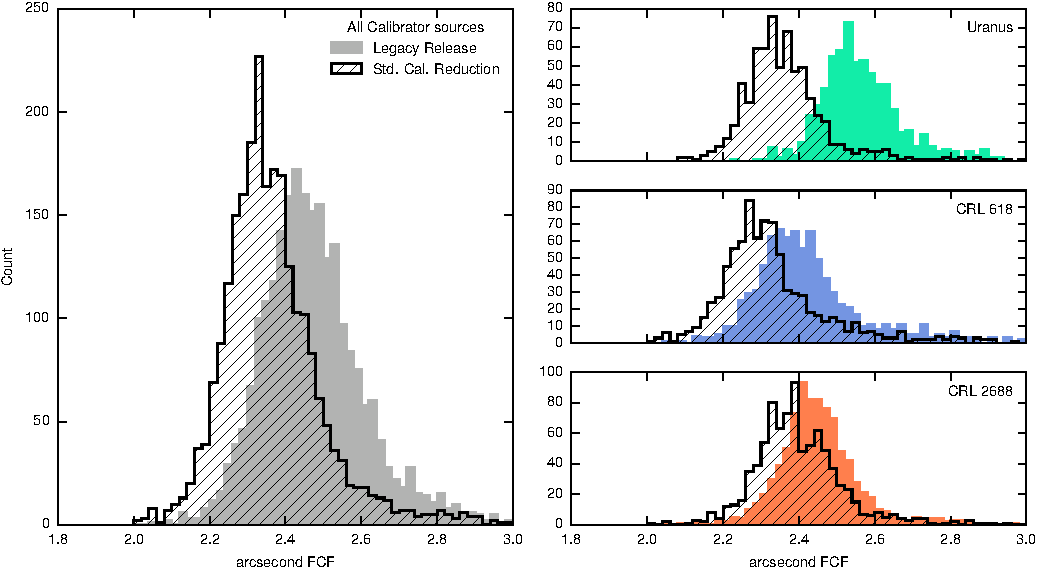
\includegraphics{legacyFCF-caldbFCF-histograms.pdf}
% \caption{Comparison between the histograms of
%   arcsecond FCFs derived from the legacy reduction and the standard
%   JCMT SCUBA-2 calibrator reduction, for the same observations.
%   These are shown both overall and broken down by source (CRL\,618,
%   CRL\,2688, and Uranus). Note that the LR Uranus maps were \emph{not}
%   reduced onto a HEALPix grid, but did use the same pixel area and
%   \texttt{makemap} dimmconfig as the other LR reductions.\label{fig:lr-caldb-histo}}
% \end{figure*}

% \begin{figure*}
% 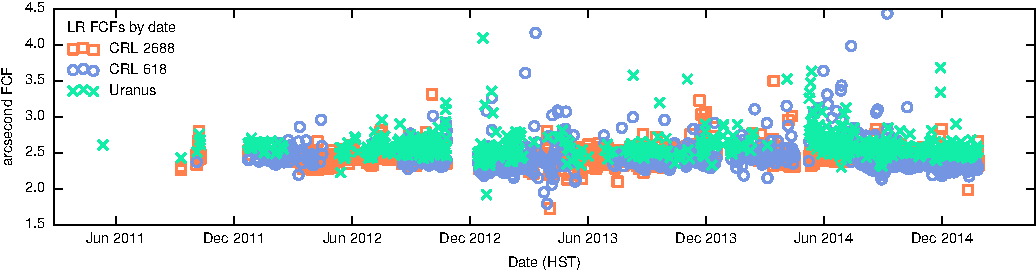
\includegraphics{legacyFCF-vs-date.pdf}
% \caption{The arcsecond FCFs derived for the legacy reductions of CRL\,618,
%   CRL\,2688, and Uranus, shown against time. Although there is a
%   large scatter and some hints of variation , it can be seen that there is not
%   clear overall dependency with time.\label{fig:calibvstime}}
% \end{figure*}

\end{document}
